%Latex Header

\documentclass[letterpaper]{report}

\usepackage{geometry}
\geometry{letterpaper}
\usepackage{multicol}
\usepackage{verbatim}

\usepackage{fontspec}
\usepackage{amsmath}
%\usepackage[MnSymbol]{mathspec}
\usepackage{mathpazo}
\setmainfont
     [ BoldFont       = texgyrepagella-bold.otf ,
       ItalicFont     = texgyrepagella-italic.otf ,
       BoldItalicFont = texgyrepagella-bolditalic.otf ]
     {texgyrepagella-regular.otf}
\setmainfont{Gill Sans MT}

\usepackage[english]{babel}
\usepackage[utf8]{inputenc}
\usepackage[colorinlistoftodos]{todonotes}
\usepackage{physics}

\usepackage{caption}
\usepackage{subcaption}
\usepackage{graphicx}

\usepackage{url}

\renewcommand{\thesection}{\thechapter.\arabic{section}}
\renewcommand{\thesubsection}{\thesection.\arabic{subsection}}
\renewcommand{\thesubsubsection}{(\roman{subsubsection})}

\title{Collaborative, Contact-Based Schemas for Robot Righting utilizing Hull Shape Design}
%Collaborative Collision- and Contact-based Schemes for Robot Roll Righting (c3r3)

\author{David McPherson}

\date{Autumn 2017}

\begin{document}

\maketitle
\global\csname @topnum\endcsname 0
\global\csname @botnum\endcsname 0

\begin{abstract}
Nature's self-organizing teams have long inspired engineering researchers.
Imitating birds and fish, researchers built swarms that could keep formation via elegant decentralized control algorithms.
Inspired by ants, they applied formation keeping to carrying loads as a mobile robot team.
In this work, we further specialize this collaborative manipulation to manipulating team-mates, thereby creating collaborative locomotion.
Our design space is enriched by designing both the manipulator and the manipulatee at the same time.
Traditional collaborative manipulation work focuses on manipulating objects in the same plane of movement as the mobile robots and adheres strictly to form or force closure manipulation paradigms.
Our new design richness allows us to leverage work on in-hand, dexterous manipulation and dynamic manipulation techniques to manipulate objects (now teammates) in degrees of freedom (DOF) outside our plane of movement.
These further manipulation DOF are accessed by especial care in designing the contact surfaces between robots which allows us to guide objects while slipping, instead of rigidly demanding complete closure.
This paper will demonstrate the collaborative locomotion concept in the simplest possible cooperative maneuver: rolling a pronated robot back onto its feet (adding a previously inaccessible roll DOF to a differentially driven robot).
Within this showcase application we discover several possible designs for cooperative righting strategies.
The strategies follow the traditional manipulation classification framework: kinematic, quasi-static, and dynamic.
We investigate each method analytically as well as implementing the best method on real robots.

\begin{figure}[ht]
\centering
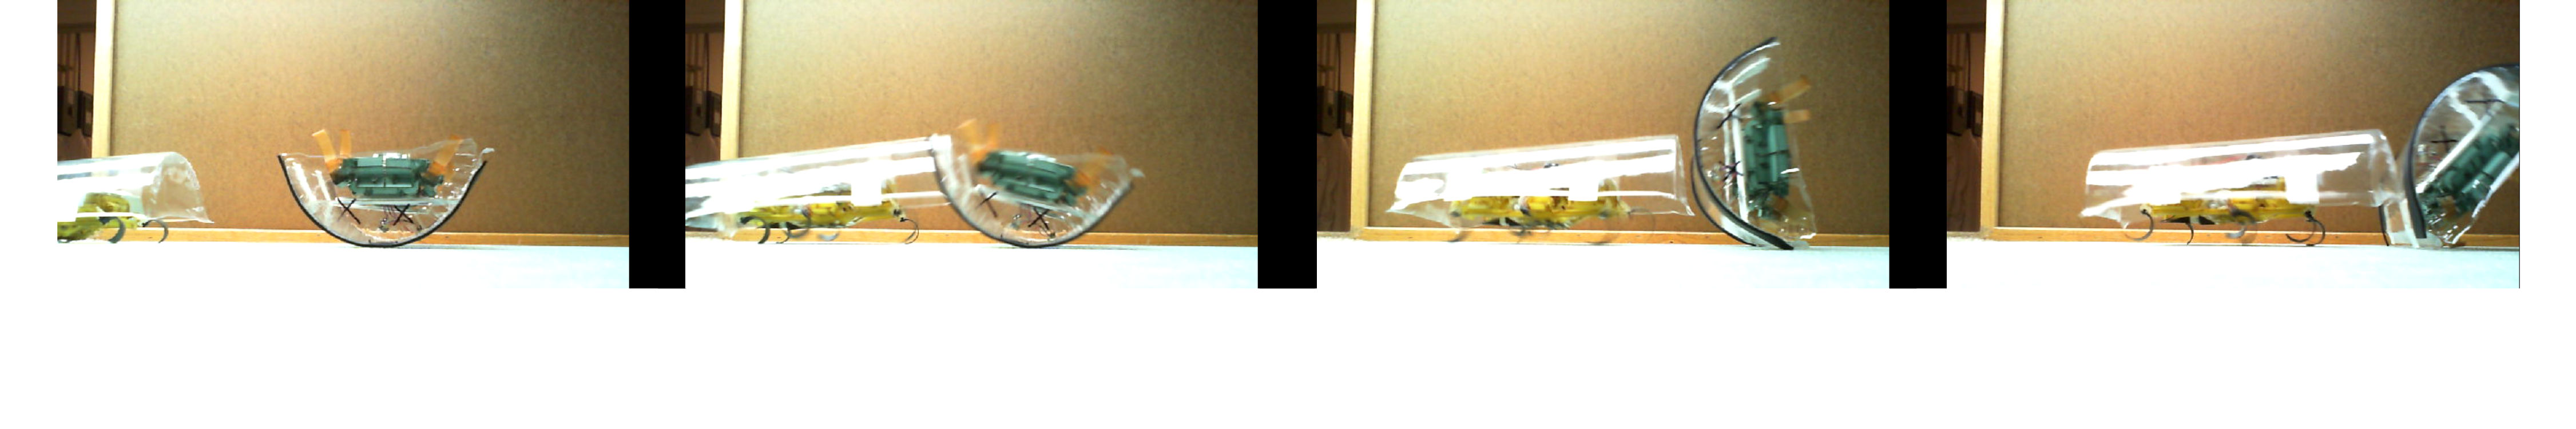
\includegraphics[width=1.0\textwidth]{QSFlipStrip3.png}
%\caption{Frame sequence of RoACH team performing our cooperative righting maneuver on styrofoam}
\end{figure}
\end{abstract}

\section{Introduction to Cooperative Locomotion}
Dolphins leaping in unison, birds soaring in tight formation, and ants carrying away feasts spark the imagination of children and engineers alike.
It should come as no surprise, then, that roboticists have striven for decades to imbue robots with that selfsame social spark.
And humanity has succeeded to some extent.
Decentralized control strategies inspired by flocks of birds \cite{reynolds1987flocks} produce tight formation controls for our flying robots \cite{RealBoids}.
This newfound capacity for formation control enabled cooperative manipulation of objects \cite{rus1995moving,sugar2002control,spletzer2001cooperative,song2002potential} just like ants \cite{kube2000cooperative}.
We take this a step further by having teams manipulate a very special object: another team member.
Inspired by self-assemblages \cite{Anderson2002} and intermediate-level parts \cite{Anderson2001} used by social insects, the team can add news modes of movement and controllable DoF for our robots.

\begin{figure}[ht]
  \centering
  \begin{subfigure}[t]{0.8\textwidth}
    \centering
    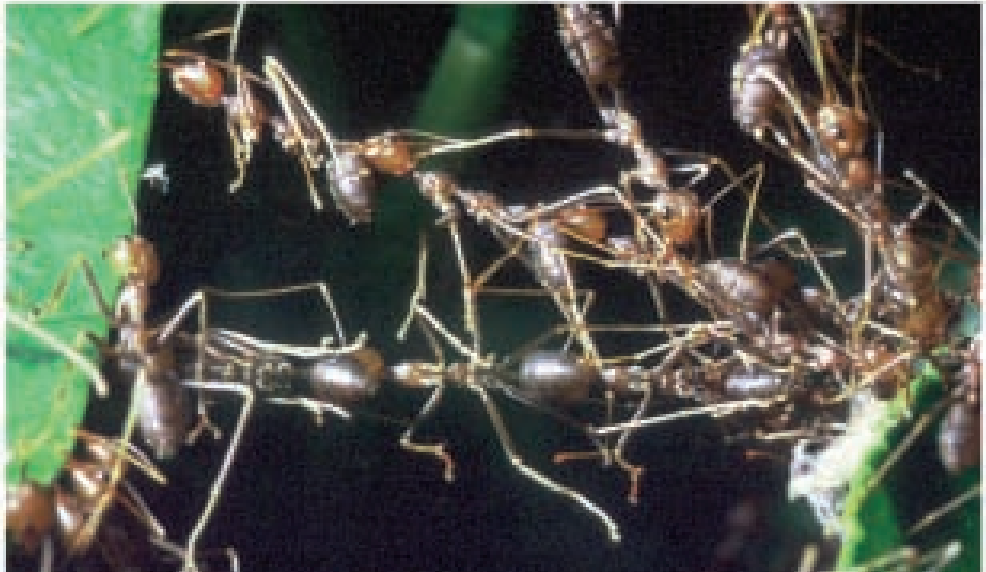
\includegraphics[width=.5\linewidth,height=.3\textwidth]{AndersonAntBridgeL.png}%
    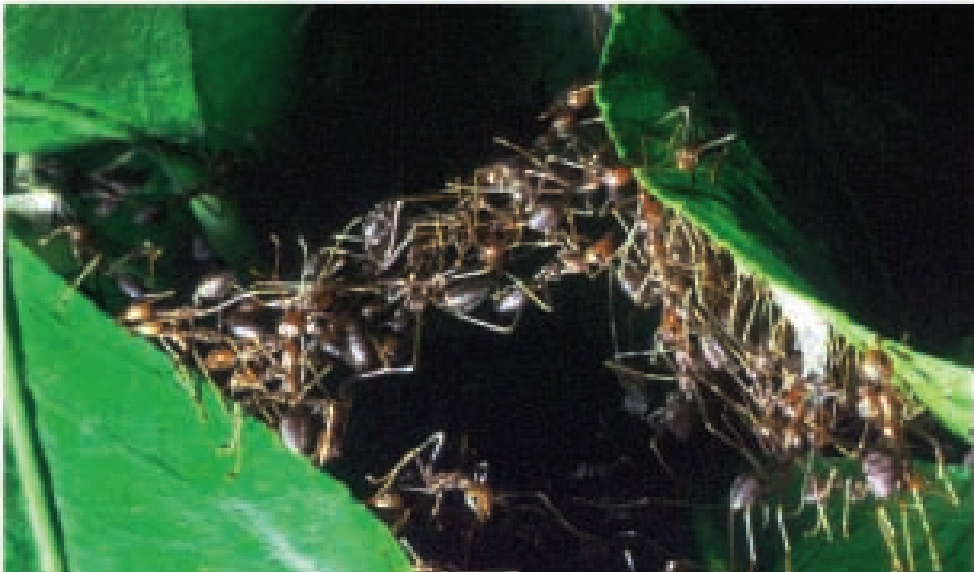
\includegraphics[width=.5\linewidth,height=.3\textwidth]{AndersonAntBridgeM.png}\\
    \caption{Army ants build bridges to cross gaps \cite{Anderson2002}}
  \end{subfigure}

  \begin{subfigure}[t]{0.8\textwidth}
    \centering
    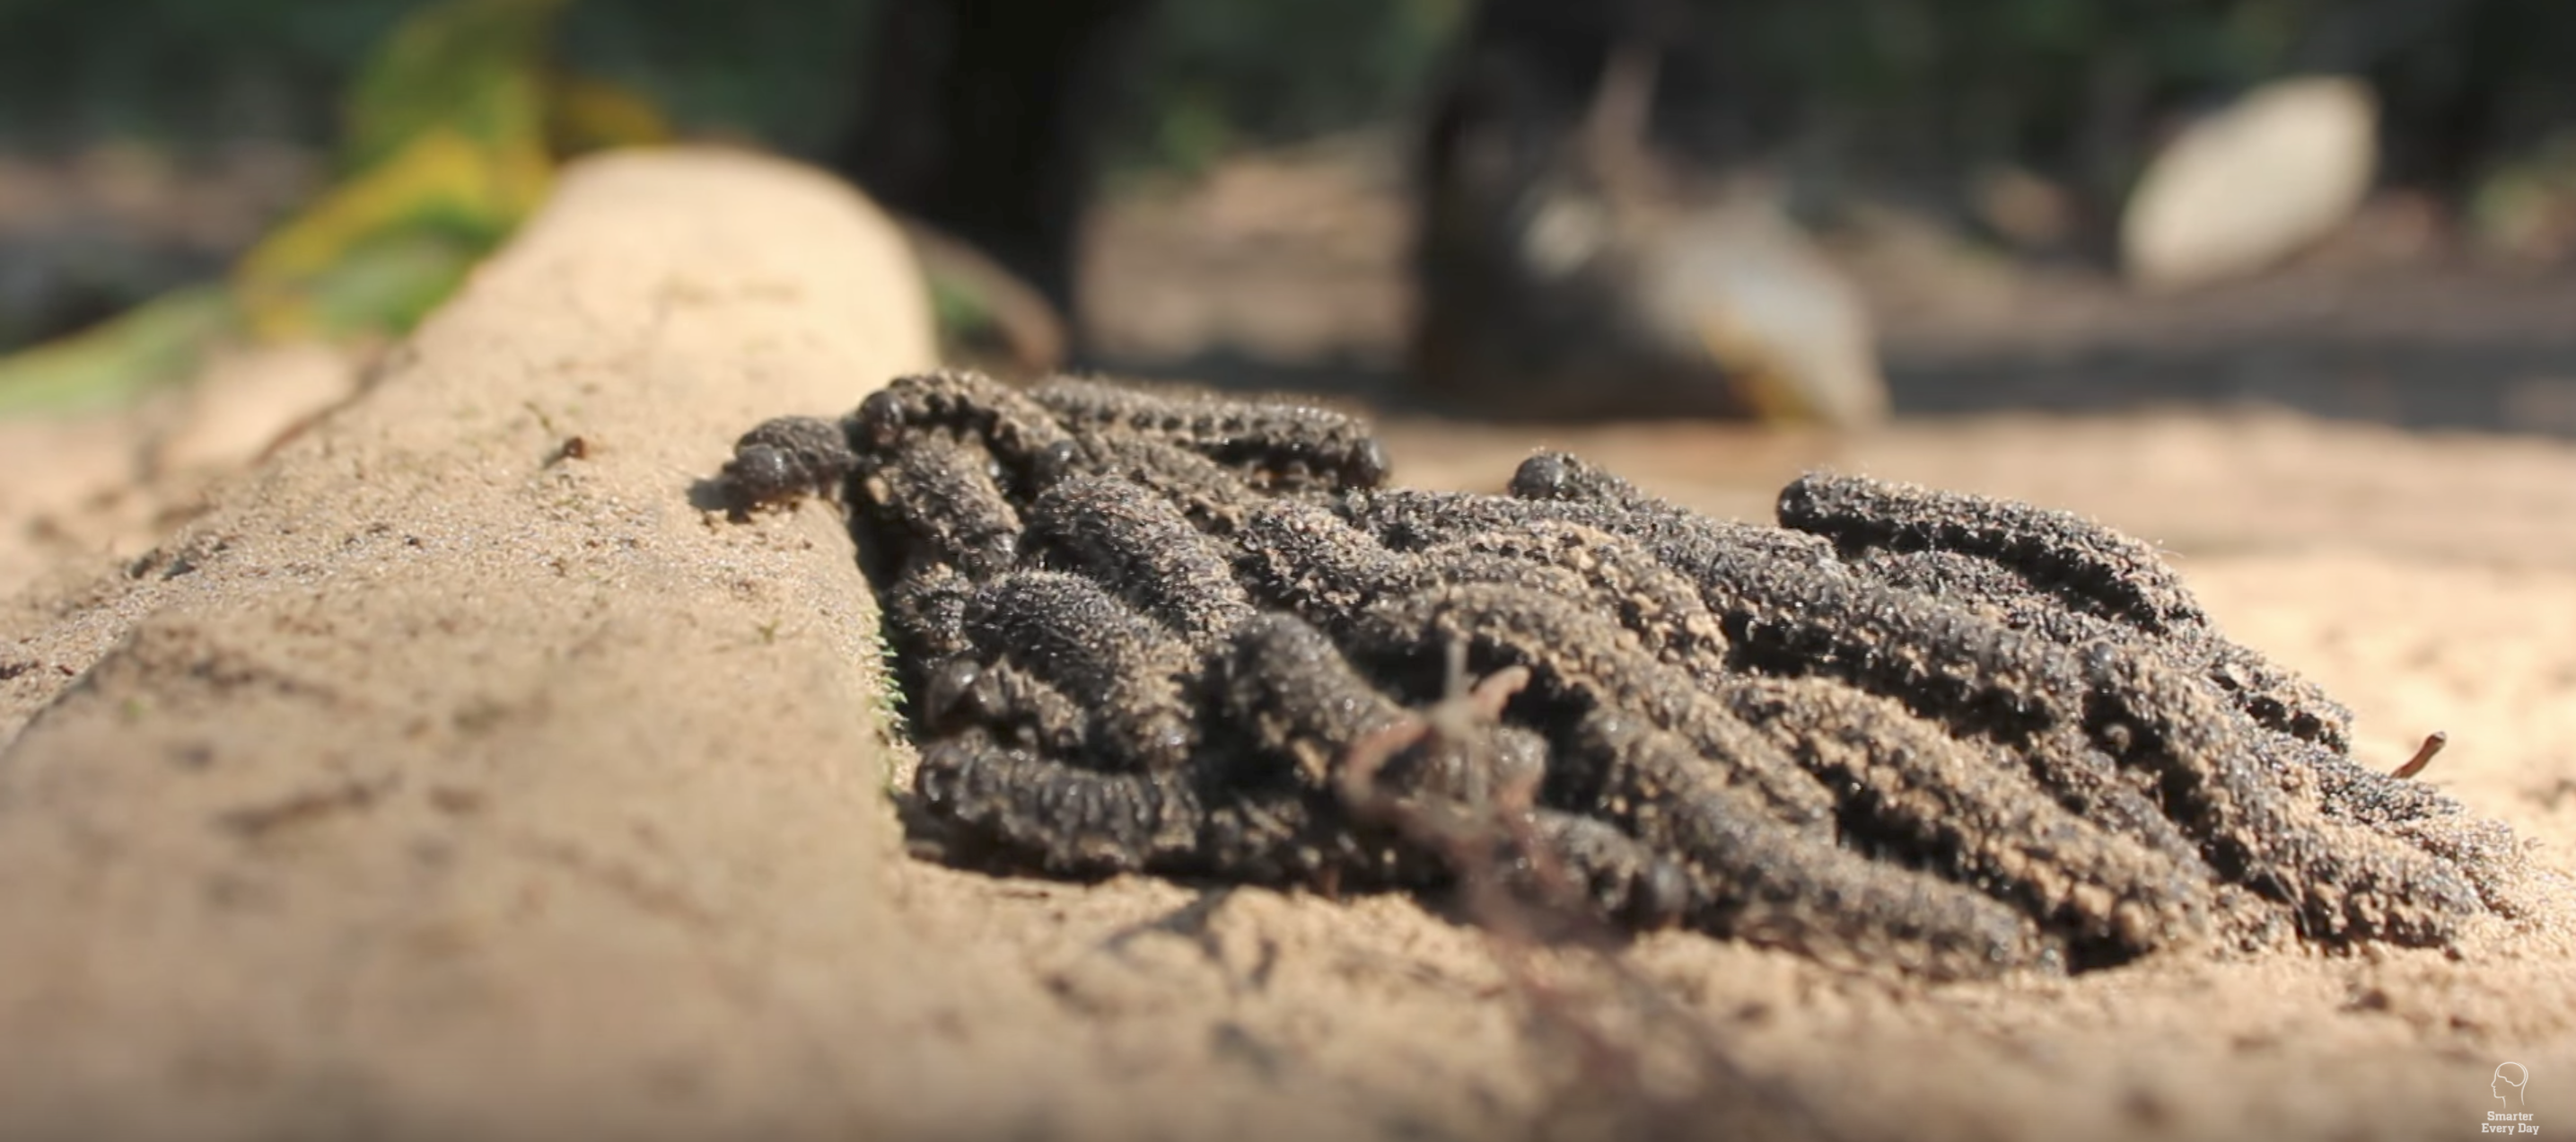
\includegraphics[width=\linewidth]{SawflyLarvaeClimb.png}
    \caption{Sawfly larvae using aggregations to boost speed and clear obstacles \cite{SEDSawflyCluster}}
  \end{subfigure}
\end{figure}

As we focus manipulation on manipulating team members, our goal is to translate work in cooperative manipulation to cooperative locomotion.
The design freedom granted by specializing manipulation to other teammates allows us to create more rich manipulations than mere translations.
By leveraging work in dynamic manipulation, we can design mobile robots that can rotate each other out of the plane of movement.

\subsection{Structure of Thesis}
This Thesis first exposits the rich tradition of research this work builds upon. This will take the rest of this chapter.
We then detail the hardware used in our experiments in Chapter 2 for the sake of reproducibility.
The next three sections each investigate a different schema for cooperative righting.
We follow the manipulation taxonomy expounded upon in Mason's seminal text ``Mechanics of Robotic Manipulation'' \cite{MasonMORMBook}: Kinematic, Static\footnote{Interestingly, static righting corresponds to passive self-righting by placing the center of gravity above the center of rotation. Static righting is non-cooperative and so doesn't receive a treatment here (static manipulation also did not receive its own chapter in ``Mechanics of Robotic Manipulation'' \cite{MasonMORMBook})}, Quasi-static, Dynamic.
Chapter 3 investigates a two robot (corresponding to a ``two-finger'' manipulation) maneuver that rolls a pronated third robot back onto its feet.
The two robots fully constrain the third robot. Closing the distance between the two robot fingers kinematically moves the third through a full roll re-orientation.
This method is purely kinematic.

\begin{figure}[ht]
\centering
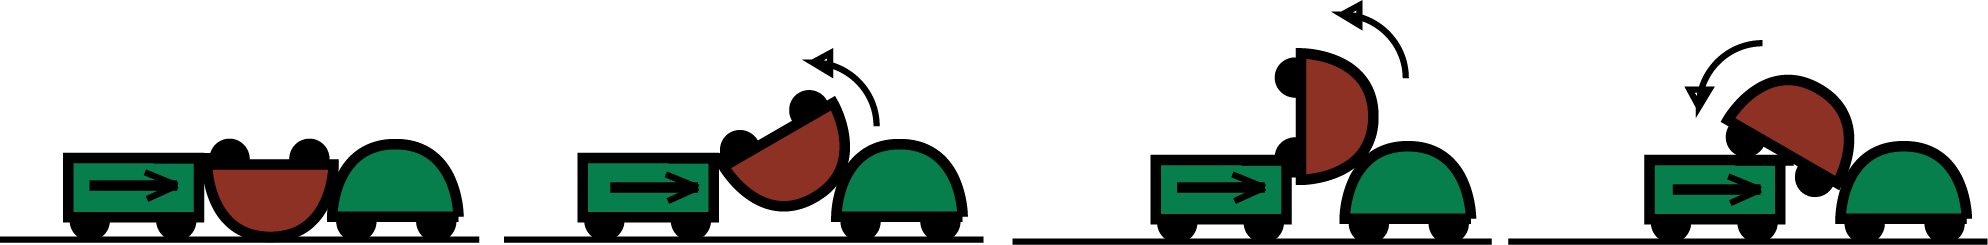
\includegraphics[width=1.0\textwidth]{Kinematic_CoopCartoon.png}
\caption{Cartoon of ``Kinematic'' Cooperative Flip Technique}
\end{figure}

Chapter 4 moves to a single robot locomoting the pronated robot. With the loss of fully constrained control, the cooperative locomotion method must compensate by leveraging previously unmodeled effects.
Previously neglected ground friction forces now become our ally providing the necessary second force to create a moment couple on the pronated robot.
In this sense the ground could be interpreted as a second finger, but is more proximal to the palm in human dexterous manipulation.
By introducing frictional forces we leave the domain of kinematic manipulation and enter quasi-static analysis, making this the quasi-static flipping method.

\begin{figure}[ht]
\centering
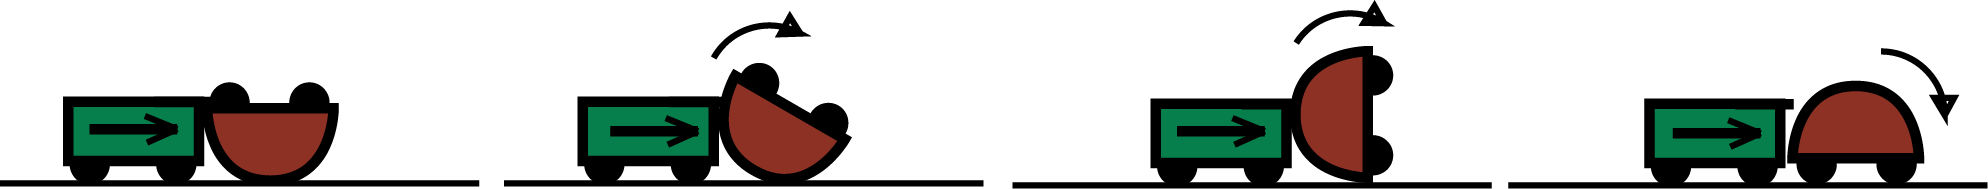
\includegraphics[width=1.0\textwidth]{QuasiStatic_CoopCartoon.png}
\caption{Cartoon of ``Quasi-static'' Cooperative Flip Technique}
\end{figure}

We will see that this enabling insight will also become the quasi-static flip's major short-coming: sensitivity to ground-shell friction coefficients.
The final flipping method eschews this constraint by relying on the inertial pseudo-force to couple with a ballistic push from the compatriot robot to create the moment couple.
This method is discussed in Chapter 5.

\begin{figure}[ht]
\centering
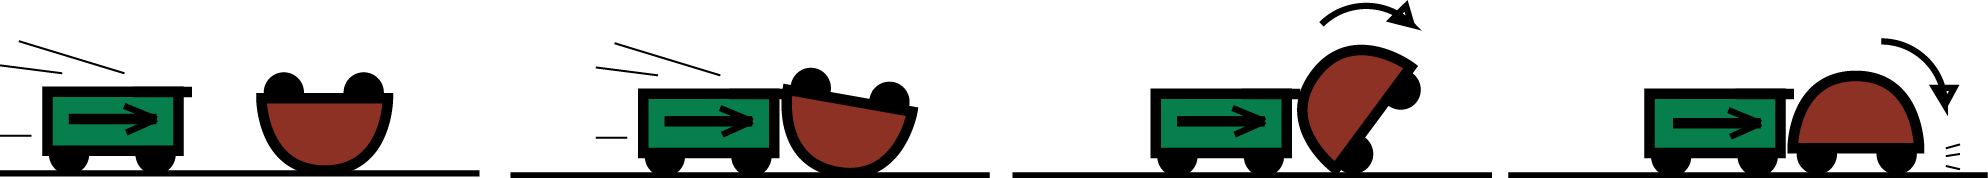
\includegraphics[width=1.0\textwidth]{Dynamic_CoopCartoon.png}
\caption{Cartoon of ``Dynamic'' Cooperative Flip Technique}
\end{figure}

Chapter 6 concludes by comparing and contrasting each cooperative righting method.
We also discuss future directions and indulge in imagining what cooperative locomotion could do after this work.

\section{Related Work}

This work is strongly rooted in the grasping and automated manipulation literary tradition.
It weds three separate branches of this rich field to investigate a new class of behaviors and manipulations.
We weave together work on cage-free manipulation, team manipulation, and self manipulation.

\subsection{Team Manipulation}
Classic grasping work focuses on placing multiple fingers to yield form closure or force closure by keeping all disturbances and wrenches within the friction cone.
Team manipulation ports these concepts by simply viewing each robot as a separate finger and using a team of mobile robots to grasp and manipulate an object.
This idea was spearheaded and popularized by Daniela Rus in her seminal work on furniture moving robots \cite{rus1995moving}.
The idea was evolved and matured by Vijay Kumar's group to include tactile feedback \cite{sugar2002control}, vision-based formation keeping \cite{spletzer2001cooperative}, and elegant decentralized control methods \cite{song2002potential}.
However, these works can only achieve manipulation within the plane that the mobile robots drive upon.
This work adds out-of-plane rolling capability to a mobile team manipulator by incorporating dexterous manipulation techniques.

\subsection{Cage-Free Manipulation}
We accomplish this feat by tapping into cage-free manipulation techniques that embrace dynamics and askew forces to create more complex manipulations.
Beautiful examples of this elegant manipulation philosophy is championed by Matt Mason's Manipulation Lab \cite{lynch1999dynamic}\cite{dafle2014extrinsic}.
My work particularly pulls upon his student Alex Rodriguez's work on shape design that molds the normal forces applied throughout a surface contact interaction to achieve the desired manipulation \cite{rodriguez2013effector}.

\subsection{Cooperative Locomotion}
Rather than manipulate arbitrary objects we investigate the exciting case of cooperative locomotion: where the manipulated object is another robot teammate.
This structure simplifies the problem by allowing us to co-design both the manipulator and the manipulatee for optimal manipulability.
To our knowledge, a manipulation-based approach to cooperative locomotion is novel.

The closest comparison are other cooperative locomotion projects such as the cooperative step climbing work by Casarez \cite{casarez2016step} where teammates boost each other via a magnetic hinge connection and pull each other up via a tether.
Biomimetic approaches such as the TERMES \cite{werfel2014designing} construction team that could collaboratively build bridges, steps, or other locomotive affordances.

\subsection{Self Righting}
In this work we focus on the cooperative locomotion example of cooperative righting.
Therefore, we should compare this work to alternative righting schemes that utilize an individual robot's spare degrees of freedom to effect a roll.
For example, Chen et al. \cite{li2016cockroach} added special purpose biomimetic mechanisms for self-righting inspired by beetles' wings.
Similarly, Casarez and Fearing \cite{casarezTailRighting} demonstrate how adding an extra motorized tail can provide a self-righting behavior.
Saranli et al. \cite{saranli2004model} use the actuators they already have to roll: by flailing the robot's legs they can induce a roll moment on the body.

\subsubsection{Rightability}
Other researchers have investigated the innate passive ability of shapes to be righted (i.e. rolled in a plane with gravity as a spanning vector).
Domokos et. al \cite{domokos2008geometry} studied nature and formulated a geometric model for rightability of turtle shells.
Kessens et. al \cite{kessens2012framework,kessens2014metric} promoted a generalized framework for analyzing robot righting using a variety of limbs and actuators.
His framework builds a graph structure on stable configurations with transitions costs weighted by change in potential energy between states.
This method is effectively a Hamiltonian analysis between discrete states (we will pursue a Hamiltonian analysis of our methods as well, but with a continuum of states instead of discontinuous transitions).
Unlike Kessens (and more like Domokos) we will doing away with added actuators and instead focusing on minimal righting strategies.
Unlike both of them we will augment the actuation with outside help from team-mates.
% TODO: Right about self-righting metrics

\chapter{Hardware}

\section{Robotic Platform}
The VelociRoACH is a Robotic Autonomous Crawling Hexapod (RoACH) experimental platform designed for high velocity running through its elegant minimal hardware design \cite{haldaneVelociRoACHDesign}.
This design makes the VelociRoACH a fertile showcase for dynamic maneuvers; it has broken speed records before \cite{haldane2015running}.
Due to its low cost and rapid manufacturing process, teams of RoACHes are a pragmatic platform for investigating multi-robot maneuvers \cite{casarez2016step}.
We will leverage these two boons to demonstrate dynamic, multi-robot maneuvers.

\begin{figure}[ht]
  \centering
  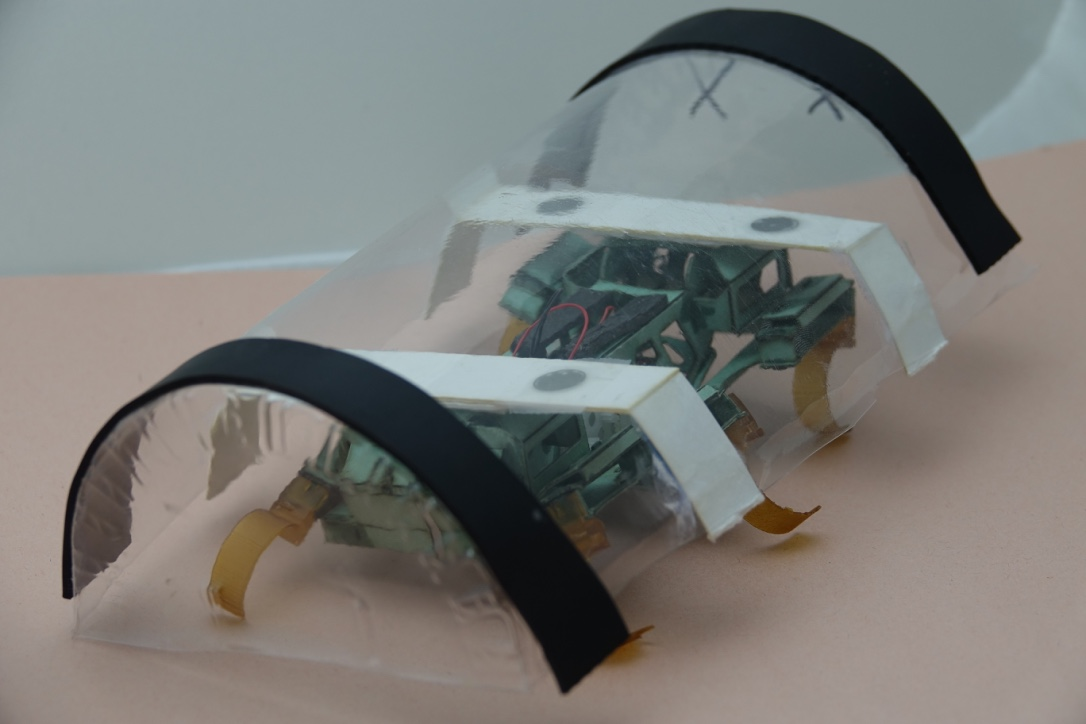
\includegraphics[width=0.8\textwidth]{ShellRoACH.jpg}
  \caption{\label{fig:ShellRoACH}VelociRoACH equipped with Roll Manipulation Shell}
\end{figure}

We accomplish our cooperative locomotion through dynamic and dexterous manipulation techniques.
These techniques rely upon molding the force vectors that are applied throughout by the manipulation contacts.
These contact forces are governed by the shape and material of the outer hull of the robot.
By adding shells to our robotic platform we can mold the reaction force landscape to suit our purposes.
This was used in Chen \cite{ChenTerradynamic} to affect how environmental obstacles push on the robot while traversing cluttered terrain.
Whereas Chen sought to use reaction forces to disengage from objects, we instead employ these forces to manipulate said objects.
Therefore, the crux of our work is designing the shell shapes for our robot.

\begin{table}[tb]
% increase table row spacing, adjust to taste
\renewcommand{\arraystretch}{1.1}
\caption{Physical Parameters of VelociRoACH and Shell}
%\vspace{-0.1in}
\label{tab:Dimensions1}
\centering
\begin{tabular}{l c c}
\hline
Parameter name & Symbol & Value \\
\hline
Body mass & $m_b$ & $54.1$ g \\
Overall width, depth, height & $(w, h)$ & $(10, 19, 10)$ cm \\
Shell circular radius & $r$ & $5.0$ cm \\
Shell major, minor axis radius & $(r, b)$ & $(5.0, 3.5)$ cm \\
Shell center offset height & $d_{circle}$ & $11.4$ mm \\
                           & $d_{ellipse}$ & $7.27$ mm \\
Shell-shell contact friction coefficient & $\mu$ & $0.52$ \\
Shell-ground contact friction coefficient & $h$ & $0.26$ \\
...with rubberized strips on shell  & $h_{rubberized}$ & $1.07$ \\
\hline
\end{tabular}
\end{table}

\section{Shell Construction}
Shell shapes are a central design problem for our application. Therefore, the design cycle of the shell is of utmost import.
To expedite the rate of design iterations, we refined the shell manufacture process by removing the primary bottleneck: speeding mold creation from days to hours.
\subsection{Mold Prototyping}
\label{sec:Molds}
Previously, in our lab we used additive manufacturing to print a mold for the shell shape.
This required multi-day printing sessions to manufacture a piece measuring 10x19x10 centimetres.
The printed thermoplastic mold would then be coated with paint so that it could withstand the molten plastic it was designed to mold in the vacuum former.
Although this method allowed nigh-infinite design freedom for shell shape, it was unacceptably slow and costly for the rate at which we needed to produce shells.
The solution we have pioneered sacrifices design flexibility for prototyping rapidity.

Our analysis will planarize the three-dimensional problem as we focus on actuating the roll degree of freedom.
Therefore, we are only interested in the two-dimensional profile of the shell and should eliminate secondary curvature along the depth-axis to prevent unwanted yaw rotations and other confounding effects.
This design goal implies that all shell designs should be prisms.
A prism's hull can be created with a single continuous sheet folded over the two-dimensional profile which defines the type of prism (e.g. rectangular prism, cylinder, elliptical prism, extruded polygon, etc.).
Constructing prismatic shells via single-sheet folding replaces the bottleneck of additive-manufacturing.

A contoured single sheet of poster-board will crumple under the vacuum pressure in a vacuum former.
We must add a supporting skeleton to brace the poster-board.
The skeleton must support pressure that points uniformly along the normals of the surface.
Since it is exerted normally, a mere square honeycomb is insufficient.
Instead, supporting beams directed along the normal must be used in the style of a Viking longhouse.
A traditional rectilinear honeycomb can then be used to supplement and hold the beams in place.
A picture of the supporting skeleton is shown in Fig. \ref{fig:ManufactureSkeleton}

\begin{figure}[ht]
\centering
\begin{subfigure}[t]{0.6\textwidth}
    \centering
    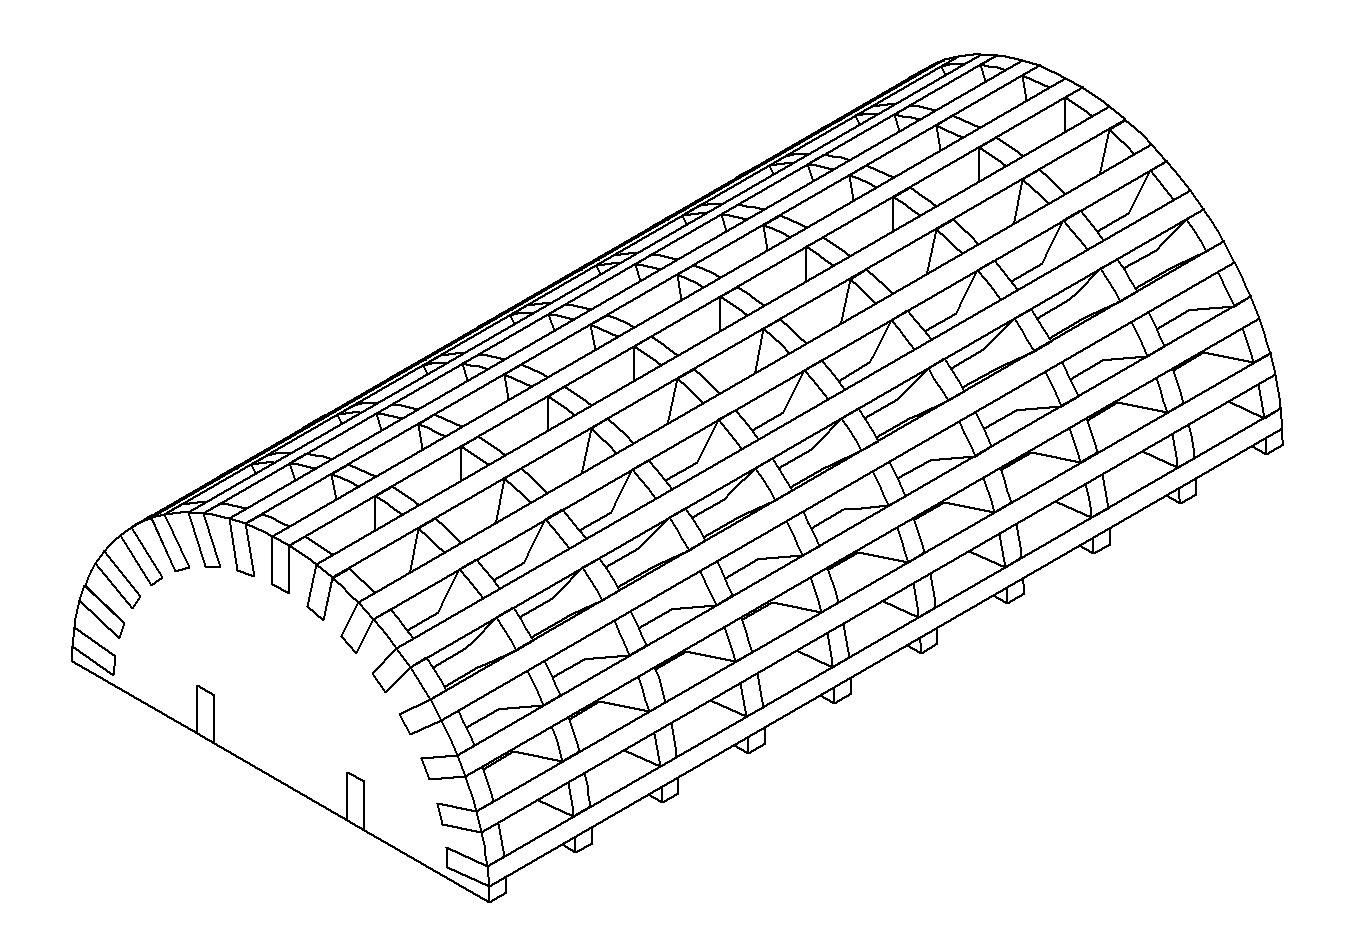
\includegraphics[width=\linewidth]{Mold.png}
\end{subfigure}
\hfill
\begin{subfigure}[t]{0.35\textwidth}
    \centering
    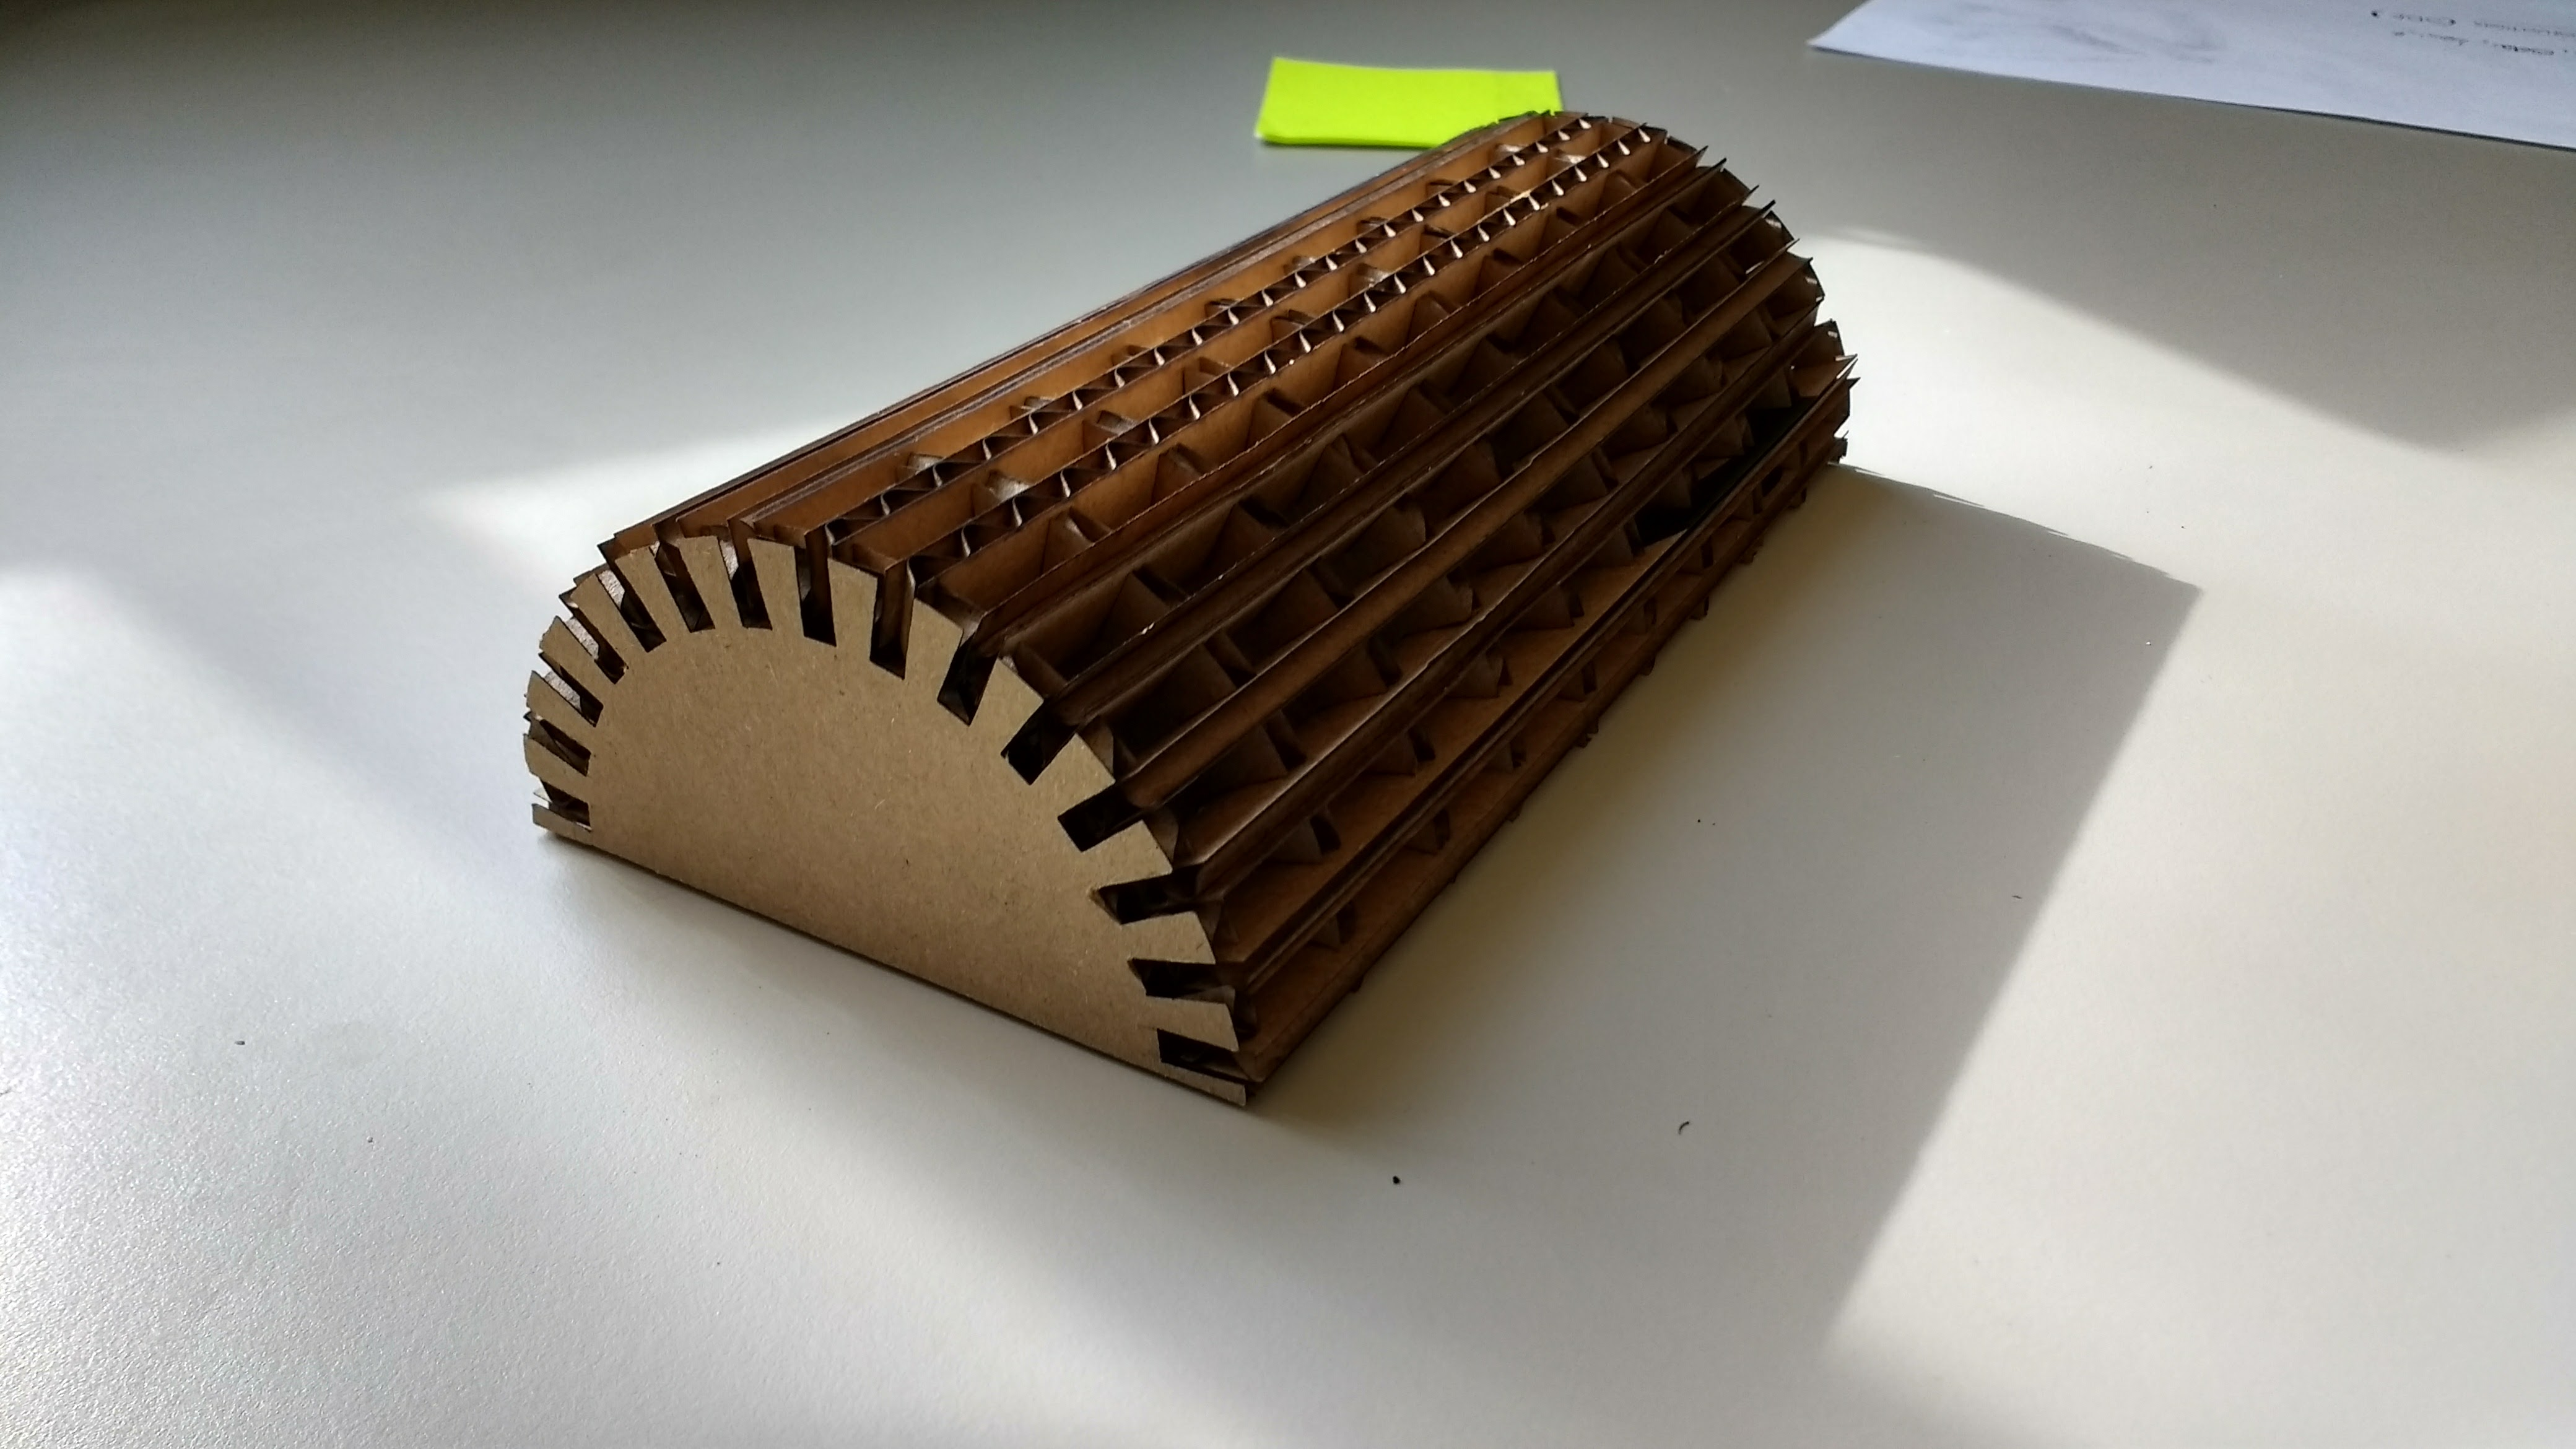
\includegraphics[width=\linewidth]{SupportingSkeleton.jpg}
\end{subfigure}
\caption{\label{fig:ManufactureSkeleton}To withstand vacuum forming pressures, the prismatic mold is reinforced with a laser cut cardboard skeleton}
\end{figure}

The poster-board can now be wrapped tightly around the supporting skeleton.
A rectangular jig cutout to fit the mold's footprint enables tight cinching and hands-free fixturing,
The skeleton is then held in place whilst the poster-board is slipped between the skeleton and the jig.
The poster-board is pulled taut (so as to avoid wrinkles forming during the suction event) and glued to the skeleton.
The completed mold is now ready to be used in the vacuum former to shape plastic shells.

\begin{figure}
\centering
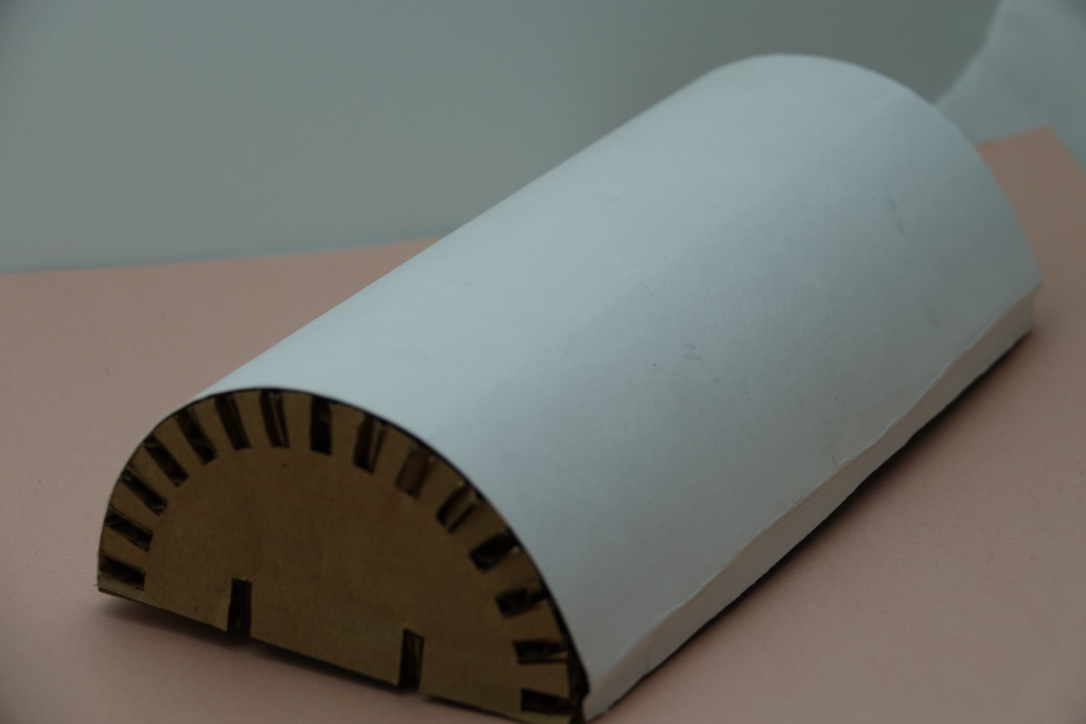
\includegraphics[width=0.8\textwidth]{FinishedMold.jpg}
\caption{\label{fig:Finished Mold}Manufactured from flat stock materials, the finished mold is ready to vacuum form plastic shells}
\end{figure}

We vacuum formed 0.015 inch thick polycarbonate to our mold using the Formech Compac Mini Vacuum Former.
The mold was constructed out of standard corrugated cardboard from recycled shipping packages, measuring between 3 and 4 millimeters in thickness (varying by package).

\subsection{An Aside on Auto-Alignment and Prismatic Shells: via Reuleaux's Method of Moment Labeling \label{sec:Reuleaux}}
Besides for simplifying both the manufacturing process and mathematical analyses, prismatic shells grant one more elegant boon: yaw control for cooperation is built into the mechanics.
A prismatic shell has a rectangular footprint projected onto the ground plane.
This footprint will govern how the robot yaws when interacting with the environment.
We find that a rectangular footprint drives the robot to align with objects (esp. other teammates) it engages with, resulting in stable pushes.
The stability of a rectangular face can be seen by applying Reuleaux's method.
Fig. \ref{fig:Reuleaux} shades areas corresponding to moment labels (green for clockwise rotations, red for widdershins rotations).
Note that for the rectangle-rectangle contact the multilateral constraint rules out centers-of-rotation between the two contacts where the moment labels contradict each other (and is labeled a mixed, muddy brown).

\begin{figure}[ht]
  \centering
  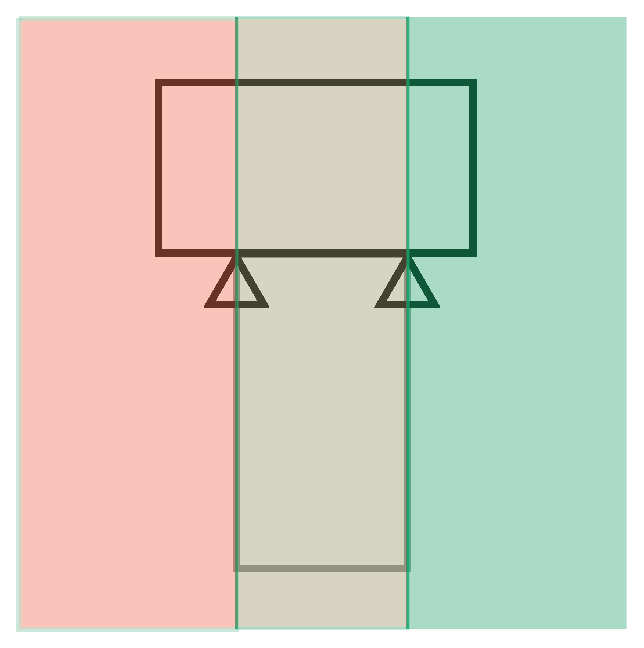
\includegraphics[height=0.3\textwidth]{ReuleauxSquare0.eps}
  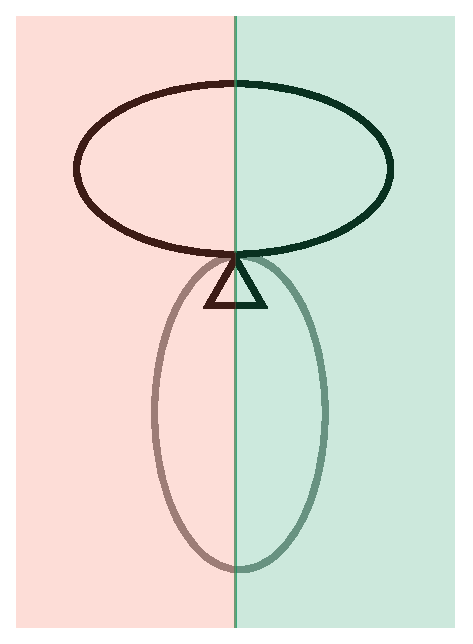
\includegraphics[height=0.3\textwidth]{ReuleauxEllipsoid0.eps}
  \caption{\label{fig:Reuleaux}Applying Reuleaux's method to contact constraints}
\end{figure}

The true stability is manifested when a second virtual finger is added: either another compatriot robot, friction (assuming weight is distributed symmetrically), or the inertial pseudo-force.
Drawing this added force on the diagram and labeling the possible moments it induces collapses the space of possible rotation centers (see Fig. \ref{fig:ReuleauxApplied}).

\begin{figure}[ht]
  \centering
  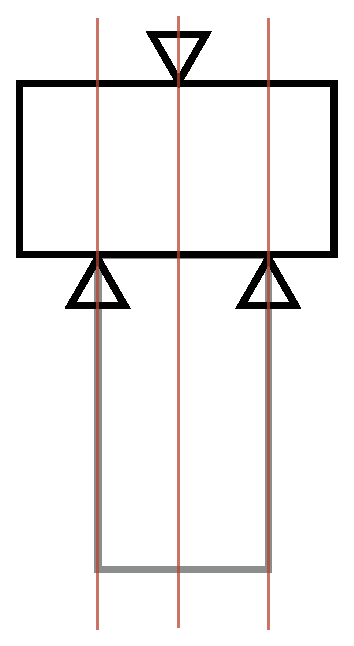
\includegraphics[height=0.3\textwidth]{ReuleauxSquare.eps}
  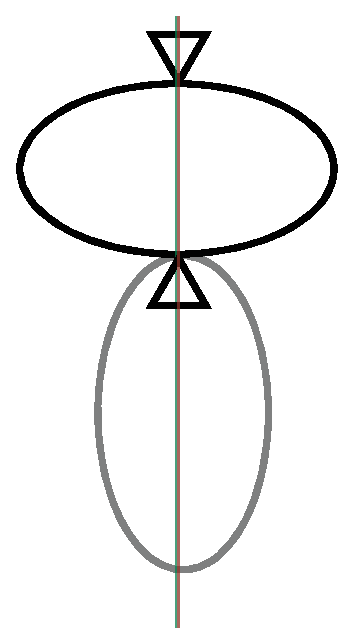
\includegraphics[height=0.3\textwidth]{ReuleauxEllipsoid.eps}
  \caption{\label{fig:ReuleauxApplied}Improved interaction stability between rectangular footprints over ellipsoidal footprints}
\end{figure}

The prismatic shells have full force closure and a firm grasp in the yaw axis.
In contrast, the ellipsoidal shells (the previous art for RoACH shells) still has infinitely many possible rotation centers: confined now to the line through both centers (in the best case) or the area between the centerlines if the pusher is even slightly misaligned.
Therefore, by Reuleaux's method, the prismatic shells have a stable grasp while the ellipsoidal grasps are an unstable equilibrium.

Leading into these grasps, too, the prismatic shells are more stable.
If the two rectangles are rotationally offset upon first contact, only one corner of the pusher will touch the prone robot.
Depending on which side of the center of friction (for quasi-static virtual finger)/center of mass (for dynamic virtual finger)/contact interval (for kinematic virtual finger) this initial touch point is on, the pusher is stably pulled into either a perfectly parallel or perpendicular configuration.
In contrast, if the ellipsoidal shells are rotationally offset upon first contact, the pusher is deflected away from their compatriot and no (even unstable) grasp is achieved.
This deflecting behavior was the original appeal of the ellipsoidal design in Chen's work \cite{ChenTerradynamic}, which refered to this effect as ``terradynamic streamlining".
In our application, however, we don't want to dodge the environment: we wish to grapple with it.
Therefore, a prismatic shell design is the most judicious choice.

\subsection{Standard Magnet Mount}
Once the plastic shells are formed to the desired prismatic shape, they are mounted to the robot via modular magnetic mounts (this allows swapping shells between experimental conditions).
The magnetic mount is a strip of poster-board strung across a horizontal secant in the shell with magnets interference fit into the top surface.
glued to the lower $\pi/6$ radians of the semi-circle
A poster-board strip is cut to length according to the formula:

$$
l_{mountstrip} = 2 \sqrt{r^2 - h_m^2} + 2 r \sin^{-1}(h_m/r)
$$

where $h_m$ is the height in the shell we aim to mount the robot.
For our experiments we choose $h_m = r/2 = 25$ mm resulting in:

$$
l_{mountstrip} = 2 (\sqrt{3} \frac{r}{2}) + 2 (\frac{\pi}{6} r) = (\sqrt{3} + \frac{\pi}{3} ) r
$$

We chose $h_m = 25$mm which mandated that $l_{mountstrip} = 139$ mm.
A second layer of poster-board measuring $\sqrt{r^2-h^2}$ is added to reinforce the unsupported horizontal secant.
This reinforcement layer also has two 9.5 mm diameter holes cut 24 mm from the centerline (center to center) to house the 3/8" diameter N52 grade magnets (1/32" deep).

The strip was then affixed to the shell via permanent adhesive. The adhesive used was LOCTITE495 Instant Adhesive.
See Fig. \ref{fig:ShellRoACH} for picture of mounted shell.





\chapter{Kinematic Flip Method}
\begin{figure}[ht]
\centering
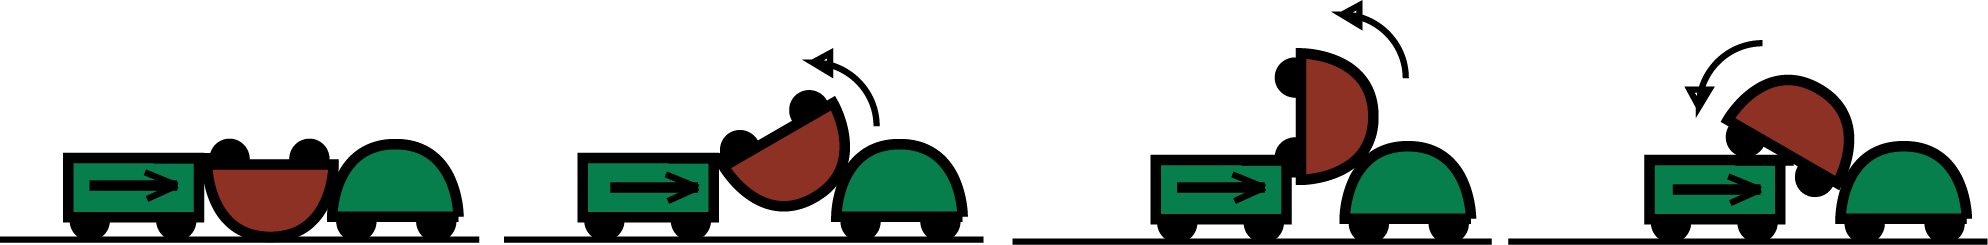
\includegraphics[width=1.0\textwidth]{Kinematic_CoopCartoon.png}
\end{figure}

The first cooperative righting method considered begins at the lowest rung on manipulation taxonomy espoused in \cite{MasonMORMBook}: kinematic manipulation.
This is the natural place to begin our translation from cooperative manipulation to cooperative locomotion since kinematic methods are the most prevalent and applied manipulation technique.
Form closure and its derivative force closure guarantee a grasp upon an object.
With object position fully determined by the manipulator, manipulation reduces to the Piano Movers' Problem in position-space for form closure or in expanded state spaces to match the dependencies of the force for force closure.

We use two compatriot robots to right the pronated team-mate. This couple kinematically constrains the manipulatee in the plane (we assume a pivot contact and a sliding contact).
Accordingly the pronated robot's pose is dictated entirely by problem geometry and evolves kinematically (independent of inertia and frictional forces).
Yet even in this simplified analysis we must still carefully design the robots' shape. Without this consideration our cooperative manipulator can only manipulate in the same degrees of freedom as the manipulators (the robot ``fingers'') can move in.
%Yet even in this simplified domain, we must still carefully carve the curves of our carriers' carcasses to caress the crabbed creation.
We draw inspiration from Zhang and Goldberg \cite{zhang2002gripper} which used a set of point contacts to rotate the manipulatee out of the plane of manipulator movement (in this case 1DOF parallel-jaw grippers).
Drawing on work by Rodriguez et. al \cite{rodriguez2013effector} we move from a set of point contacts to designing contact surfaces.

\section{Surface Design}
Inspired by parallel-jaw grippers, the action of flipping will be caused by closing the distance between two compatriot robots.
We treat one contact as a hinge joint between the compatriot and the manipulatee.
The hinge assumption holds approximately in experiments due to friction aided by a lip that catches the edge of the pronated robot and prevents sliding upwards.

The compatriot robots can either be parallel to the pronated manipulatee or perpendicular, resulting in two unique profiles in the planar manipulation problem.
When perpendicular, the prism's flat front face pushes the manipulatee. This is the face we attach that acts as a hinge (courtesy of friction and an added lip).
When parallel, the prism's long extruded profile meshes the matching profile of the pronated robot. This is the shape we get to design.

\subsection{Relative Movement}
The closing motion of our jaw-gripper-like robots is actually due only to the motion of the perpendicular robot, as our non-holonomic robots are constrained to Dubins-car-esque movements.
To simplify analysis, however, motions are generally described as the curved profile (parallel robot) moving and the hinge (perpendicular robot) remaining fixed.
Since we eschew inertial analyses in Kinematic manipulations, these reference frame simplifications present no issues.

\subsection{Shape for Contact Problem Formulation \cite{rodriguez2013effector}}
We will formulate the design problem as a shape for contact problem as advanced by Rodriguez et al\cite{rodriguez2013effector} using his three main concepts:
\begin{itemize}
  \item \textit{Motion} $\mathcal{M}(z,u)$ and \textit{Motion Orbits} that define the movement of the effector
  \item \textit{Effector} $E(s,u)$ with \textit{shape} $E(s,0)$
  \item \textit{Contact Constraints} $(p,\omega)$ and its decomposition into \textit{Shape Constraints} $((p,u),\omega)$
\end{itemize}
In our formulation, however, we are simultaneously designing the effector and the effected object each with their own \textit{motion} creating, in effect, two coupled shape-for-contact problems.
The pronated robot hinges about the perpendicular compatriot robot's lip, resulting in the \textit{motion field} $\mathcal{M}(z,u)$:

\begin{align}
\mathcal{M}_{rot}(z,u) = \begin{bmatrix} -z_2 \\ z_1 \end{bmatrix} \frac{d\theta(u)}{du}
\end{align}

where $u$ parametrizes the motion\footnote{$u$ can be thought as an analogue to the time index. But since dynamics are neglected we are actually free to choose our parameter $u$ to be some other, more relevant variable that is one-to-one with time, such as closed distance between the ``parallel jaws'' $x$ or righting angle $\theta$}
 and $z$ is the position with origin placed at the hinge as shown in \ref{fig:rotMot}
The \textit{motion orbits}\footnote{\textit{motion orbits} are a central concept in Rodriguez' formulation \cite{rodriguez2013effector}. Mathematically, they are the integral curves of the \textit{motion} $\mathcal{M}(z,u)$. Physically, they represent the path a point on the designed shape follows throughout the motion. Solutions are obtained by propagating constraints backwards along orbit lines. \textit{Motions} $\mathcal{M}$ can be $u$-varying and nonlinear, in general, and oft-times create more rich \textit{motion orbits} than the simplifed ones seen here.}
 of the hinging motion, which are the concentric circles around the hinge.

 \begin{figure}[ht]
   \begin{subfigure}[t]{0.5\textwidth}
     \centering
     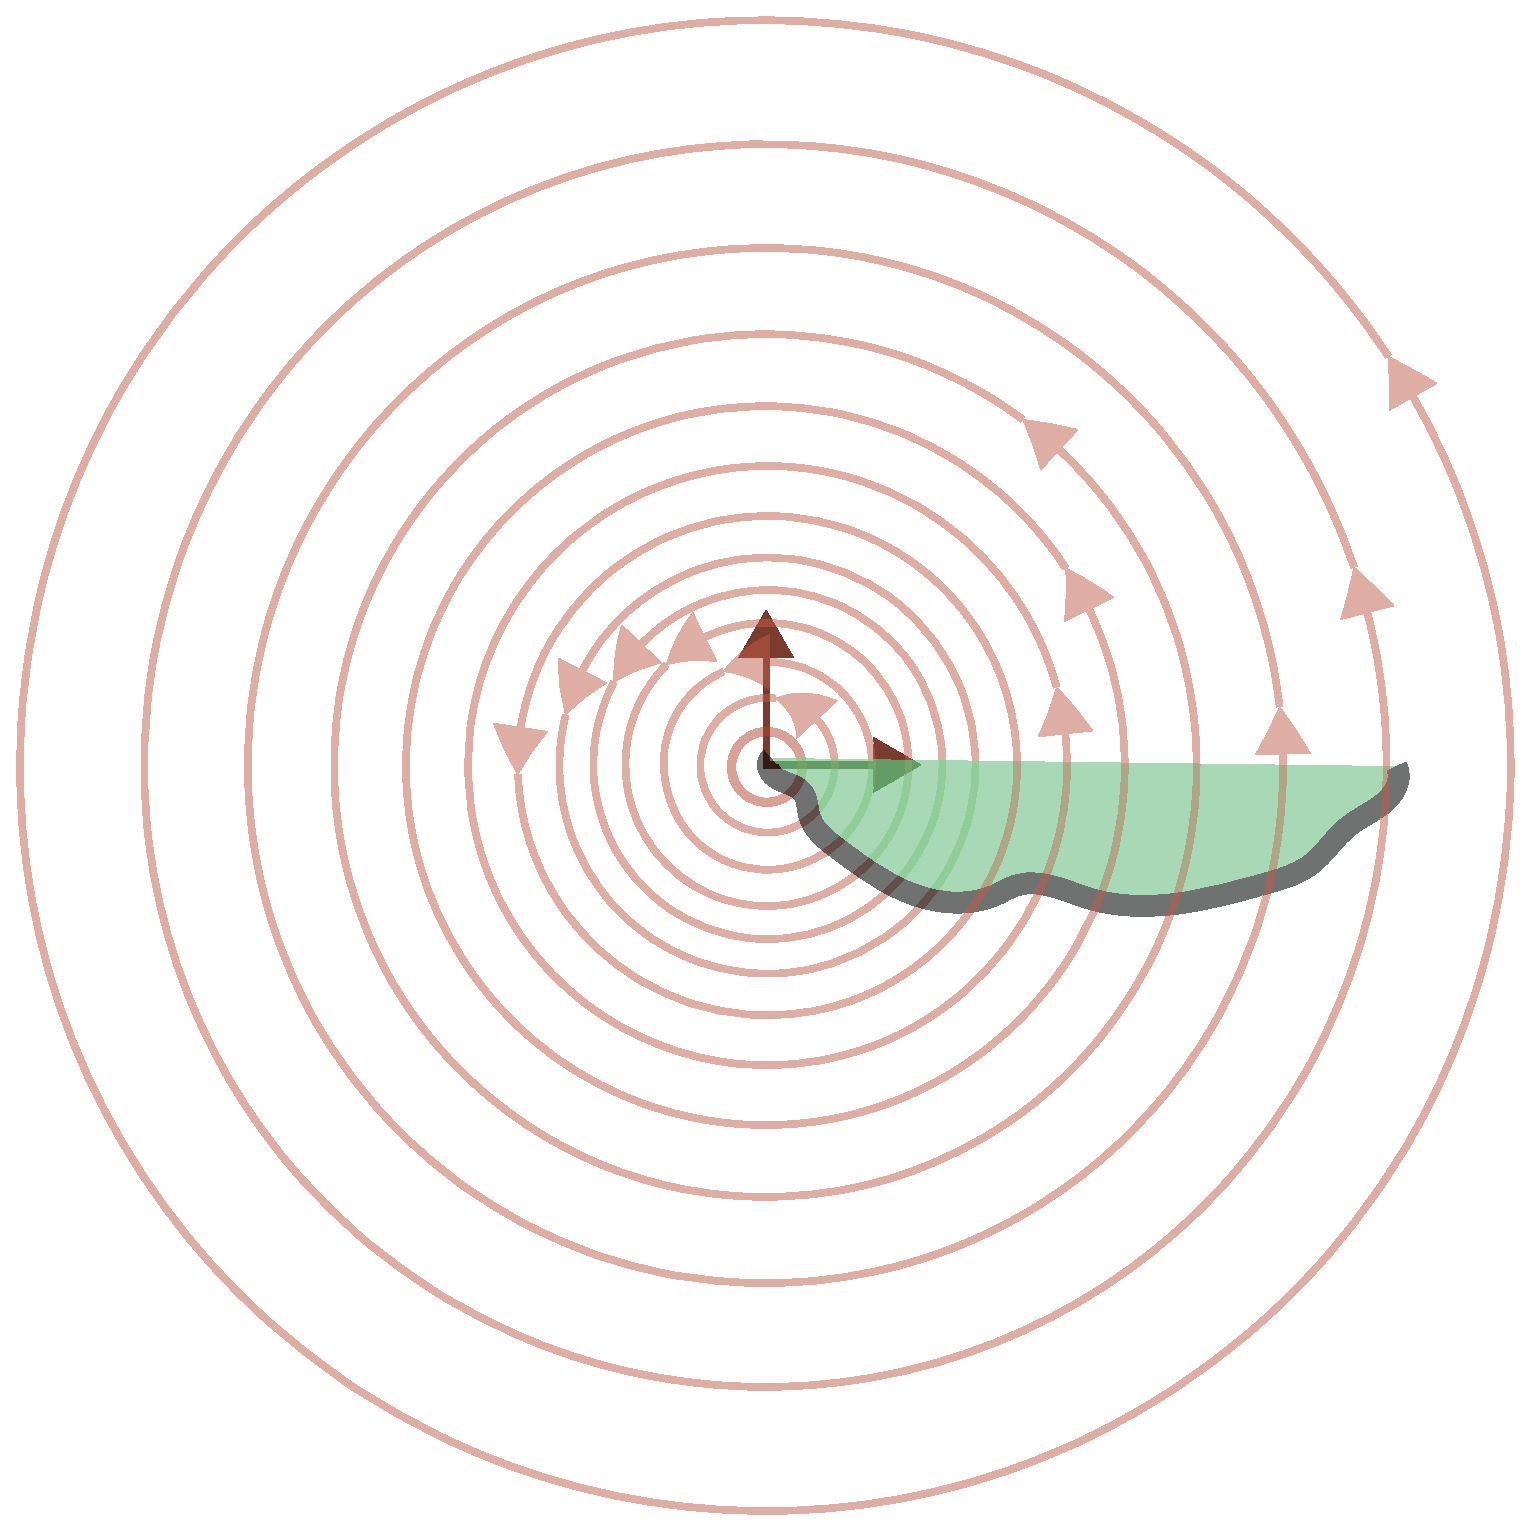
\includegraphics[width=\linewidth,trim={10cm 5cm 0 5cm},clip]{ShapeForContact_hinge2.eps}
     \caption{\label{fig:rotMot}Motion Orbits of Pronated Copy of Shell under Hinge Effector}
   \end{subfigure}
   \begin{subfigure}[t]{0.5\textwidth}
     \centering
     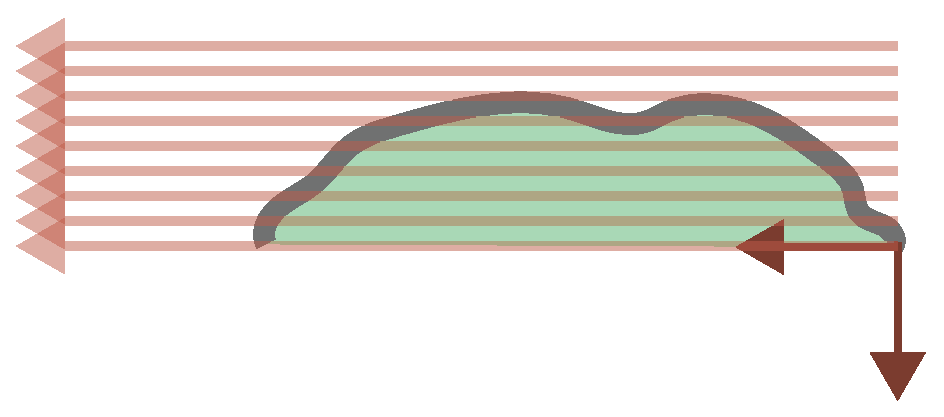
\includegraphics[width=\linewidth]{ShapeForContact_jaw.eps}
     \caption{\label{fig:transMot}Motion Orbits of Parallel Compatriot Copy of Shell under Squeeze Effector}
   \end{subfigure}
 \end{figure}

The coupled problem investigates the relative motion of the parallel compatriot robot: a closing gap, mimicking parallel jaw grippers, that pushes the prone robot up and over.
Therefore, the compatriot robot translates purely sideways with \textit{motion field}:

\begin{align}
\mathcal{M}_{trans}(z,u) = \begin{bmatrix} 1 \\ 0 \end{bmatrix} \frac{dx(u)}{du}
\end{align}

and corresponding \textit{motion orbits}, shown in Fig. \ref{fig:transMot}, being the horizontal lines.
Note that this motion has a separate coordinate frame for measuring movement.
Points can be transformed between the two coordinate frames via the affine transformation:

\begin{align}
 z_{rot}=-z_{trans}+\begin{bmatrix}w \\ h\end{bmatrix}
\end{align}

where $w$ is the starting distance between the two compatriot robots and $h$ is the height of the hinge.

Note that $\frac{d\theta(u)}{du}$ and later $\frac{dx(u)}{du}$ (referenced in the motion orbits) are design inputs chosen at the discretion of the designer.
One of the mappings between position states and motion parameter will be decided by defining the motion parameter $u$, while the other can be designed to create a (in some sense) optimal motion.
For example, we could define $u=\theta$ and choose $x(u)$ to minimize peak power consumption by letting $x(u) = w + T \sin(u)$.

We will use these \textit{motion orbits} to propagate back contact points to build out the tangent planes of our designed surface $E(s,u)\rvert_{u=0}$ (where $s$ parametrizes the curve).
Rodriguez' Shape for Contact Problem is formalized by defining the desired contact points through contact constraints $\exists u_0 \ni E(s_0,u_0) = p \and \frac{\partial E}{\partial s}(s_0,t_0) = \omega$ and shape constraints $E(s_0,u_0) = p \and \frac{\partial E}{\partial s}(s_0,u_0) = \omega$.
Our coupled problem is designing a singular $E(s,0) = C(s)$ from two sets of contact constraints.
Since the same shape $E(s,0)$ will be propagated through two different motion fields, we notate which motion field the shape is isometrically transformed by using a subscript.
\begin{itemize}
  \item $E_{rot}(s,u)$ denotes the copy of the designed curve that is rotated about the hinge. It is the copy of the shell worn by the pronated robot.
  \item$E_{trans}(s,u)$ denotes the copy of the designed curve that is translated towards the hinge, closing the jaw and pushing the manipulation forward. It is the copy of the shell worn by the parallel ``jaw'' robot.
  \item The two are coupled via the constraint $E_{rot}(s,0) = E_{trans}(s,0) = C(s) \hspace{5mm} \forall s$
\end{itemize}

Our contact constraints arise from our need for the prone robot be supported at every angle $\theta \in [0,\pi/2]$\footnote{after $\pi/2$ the prone robot's center of gravity is over the support point at the hinge, so gravity will finish the rotation work as the robot falls feet first towards the ground.}.
Supporting the prone robot means that there exists a contact point with matching tangents between the rotating copy of the curve and the translating copy of the curve.
Therefore, (translating between the two reference frames) the shape constraints must match:

\begin{align}
  E_{rot}(s_{0r},u) = -E_{trans}(s_{0t},u) +\begin{bmatrix}w \\ h\end{bmatrix} \\
  \frac{\partial E_{rot}}{\partial s}(s_{0r},u) = - \frac{\partial E_{trans}}{\partial s}(s_{0t},u)
  \label{eq:ShapeConstraintsE}
\end{align}

for some $s_{0r},s_{0t}$ for all $u \ni (\theta(u) \in [0,\pi/2])$.
By transforming the cloned curve $C(s)$ according to the motion orbits, we can substituting the coupling constraint $E_{rot}(s,0) = E_{trans}(s,0) = C(s)$ into \ref{eq:ShapeConstraintsE} to find:

\begin{align}
  R(\theta(u) ) C(s_{0r}) = - \left(C(s_{0t})+\begin{bmatrix}x(u) \\ 0\end{bmatrix} \right) +\begin{bmatrix}w \\ h\end{bmatrix} \label{eq:ShapeConstraints1} \\
  R(\theta(u) ) \frac{d C}{d s}(s_{0r},u) = - \frac{d C}{d s}(s_{0t})
  \label{eq:ShapeConstraints2}
\end{align}
where $R(\theta) = \begin{bmatrix} \cos(\theta) & -\sin(\theta) \\ \sin(\theta) & \cos(\theta) \end{bmatrix}$ is the rotation matrix through angle $\theta$.

Therefore, our task is to come up with three functions $C(s), s_{0r}(u), s_{0t}(u)$ that will satisfy the Eqs. \ref{eq:ShapeConstraints1} and \ref{eq:ShapeConstraints2}.
Rather than solve this problem for a choice of $x(u), \theta(u)$, we instead posit a solution to the problem and find the $x(u),\theta(u)$ it satisfies.

\section{Kinematic Analysis of Semi-Circular Prismatic Shells}
This flipping method is termed the ``Kinematic Flip'' since the flipping action is due purely to contact constraints that geometrically force the pronated robot through a series of poses up to the tipping point.
We posit a solution to Eqs. \ref{eq:ShapeConstraints1} and \ref{eq:ShapeConstraints2} of $C(s) = r$ being a semi-circle, and will kinematically find the $s_{0r}, s_{0t}$ that make the semi-circle a solution.
Consider the geometry of the freebody diagram in \ref{fig:KinFreebody} for a given $x(u)$ and $\theta(u)$.

\begin{figure}[ht]
\centering
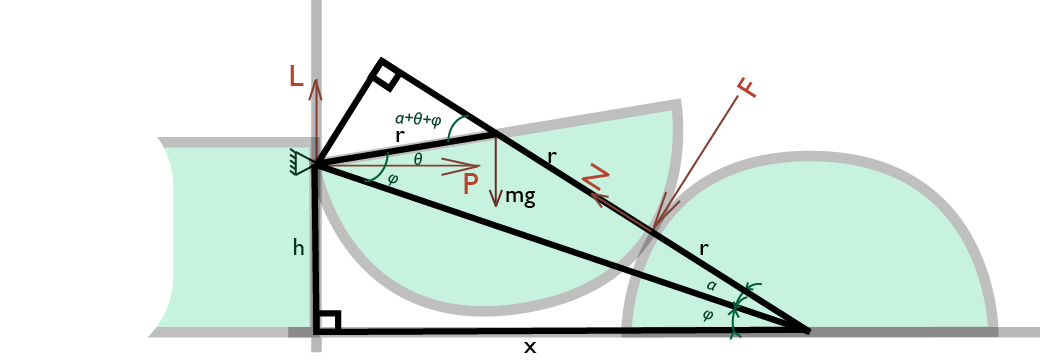
\includegraphics[width=0.8\textwidth]{Kin_FreeBodyDiagram.png}
\caption{\label{fig:KinFreebody}Freebody Diagram for Kinematic-Flip Force Analysis}
\end{figure}

We find the kinematic angles that govern this system using the law of cosines and the definition of the tangent function:

\begin{align}
  r^2 = 4 r^2 + (h^2 + x^2) - 4r \sqrt{h^2 + x^2} cos(\alpha) \\
  \rightarrow \alpha = \cos^{-1} \left( \frac{3r^2 + h^2 + x^2}{2r \sqrt{h^2 + x^2}} \right)
\end{align}

\begin{align}
  \phi = \tan^{-1}(h/x)
\end{align}

\begin{align}
  4 r^2 = r^2 + (h^2 + x^2) - 2r \sqrt{h^2 + x^2} \cos(\theta + \phi) \\
  \rightarrow \theta = \cos^{-1} \left( \frac{-3r^2 + h^2 + x^2}{2r \sqrt{h^2 + x^2}} \right) - \phi \label{eq:KinTheta}
\end{align}

Note that Eq. \ref{eq:KinTheta} creates a strict relation between $x(u)$ and $\theta(u)$.
By defining the motion parameter $u$ in terms of one, we can find the other.
Here we'll choose $x(u) = u$ so that Eq. \ref{eq:KinTheta} already expresses $\theta(u) = \theta(x)$.

With all angles kinematically defined, we pick off the contact angles $s_{0r}, s_{0t}$ as:

\begin{align}
  s_{0r}(u) = s_{0r}(x) = \alpha + \theta + \phi = \cos^{-1} \left( \frac{3r^2 + h^2 + x^2}{2r \sqrt{h^2 + x^2}} \right) + \cos^{-1} \left( \frac{-3r^2 + h^2 + x^2}{2r \sqrt{h^2 + x^2}} \right)
\end{align}

and

\begin{align}
  s_{0t}(u) = s_{0t}(x) = \alpha + \phi = \cos^{-1} \left( \frac{3r^2 + h^2 + x^2}{2r \sqrt{h^2 + x^2}} \right) + \tan^{-1}(h/x)
\end{align}

We have found a solution to the Shape for Contact problem by satisfying the constraints in Eqs. \ref{eq:ShapeConstraints1} and \ref{eq:ShapeConstraints2}: at every position $u = x$ there is a contact plane between the parallel jaw and the pronated robot.
As $x$ increases the flip angle $\theta$ also increases according to \ref{eq:KinTheta}, until the critical angle $\theta = \pi/2$ when the center of gravity crosses over the support point at the hinge.
At this critical angle the two bodies become decoupled as the prone robot breaks contact with the pusher and clatters to the ground on its feet.

\section{Experimental Results}

This semi-circular shell design was found to be kinematically successful as can be seen in Fig. \ref{fig:KinematicFlipRealLife}

\begin{figure}[ht]
  \centering
  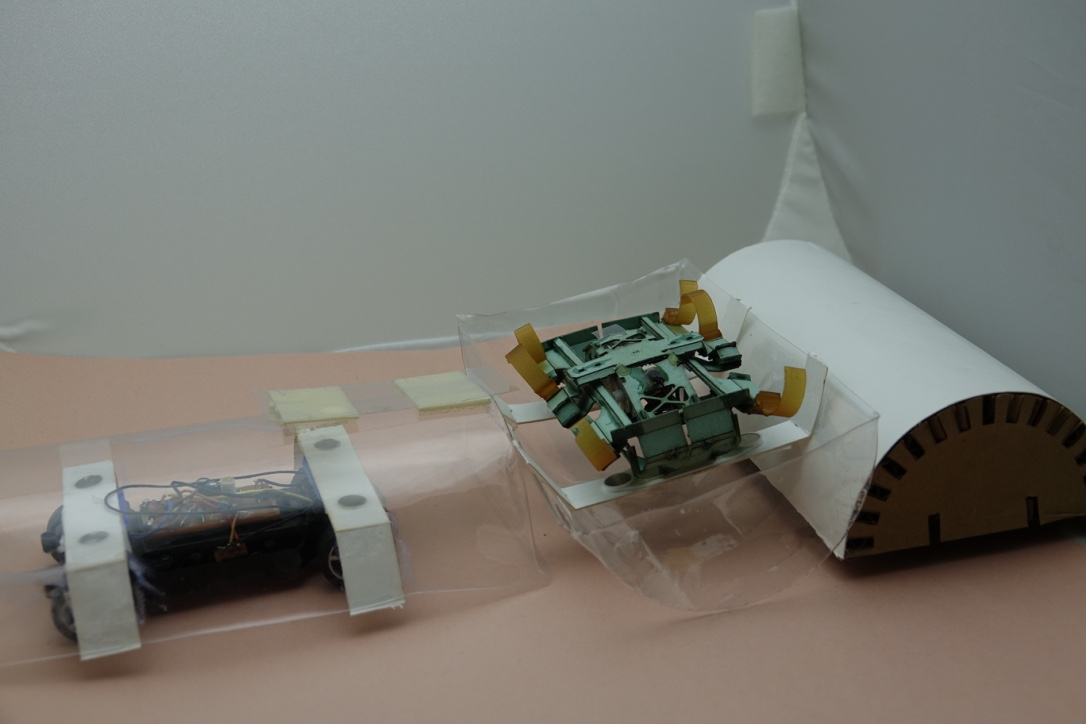
\includegraphics[width=0.16\textwidth]{KinPanel0.jpg}
  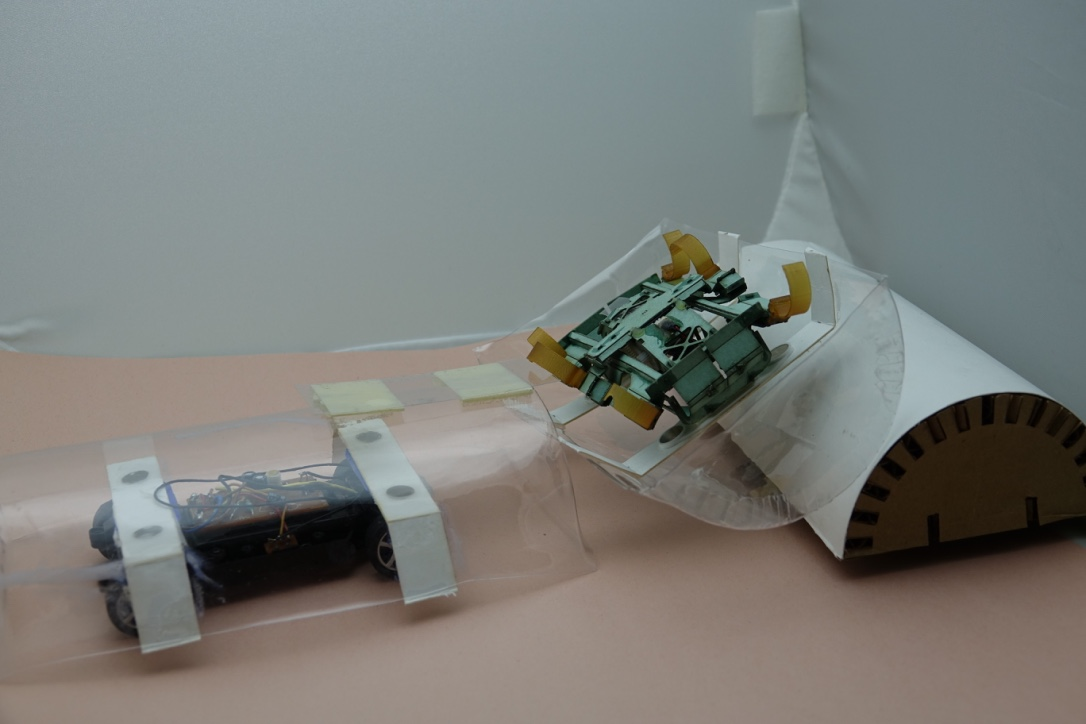
\includegraphics[width=0.16\textwidth]{KinPanel1.jpg}
  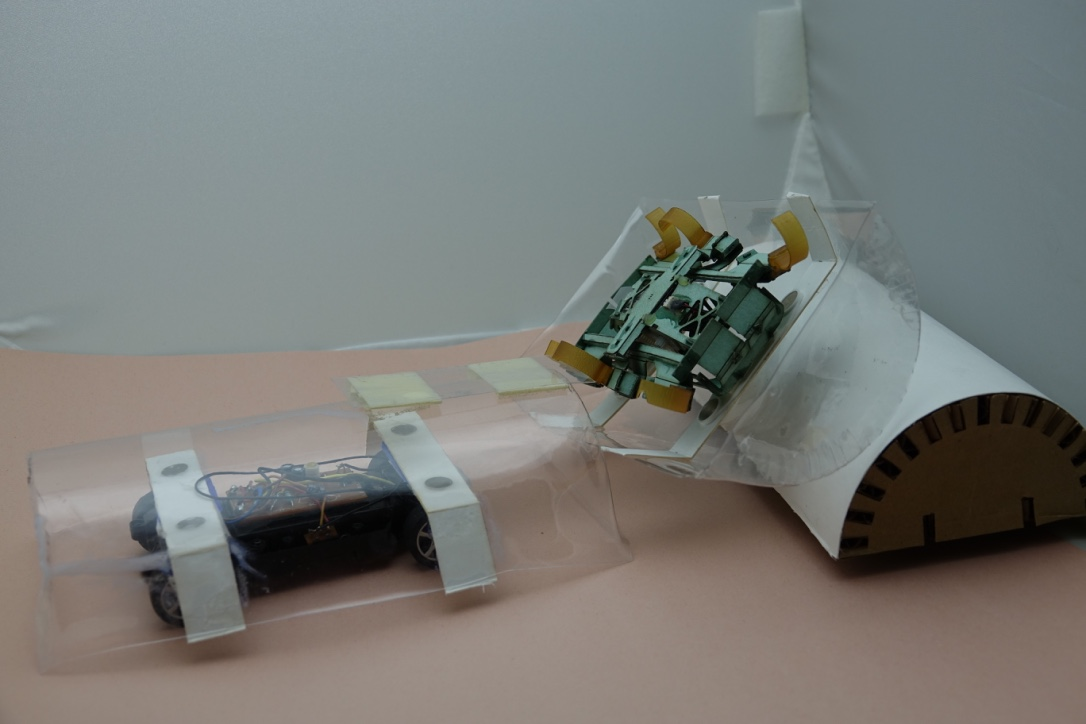
\includegraphics[width=0.16\textwidth]{KinPanel2.jpg}
  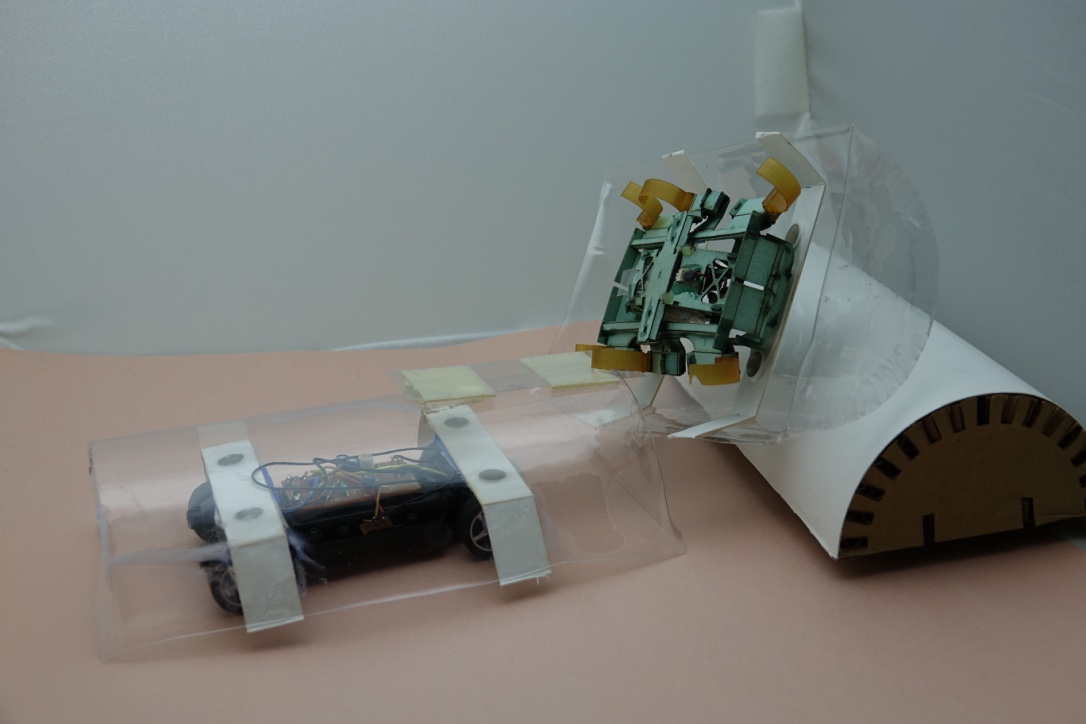
\includegraphics[width=0.16\textwidth]{KinPanel3.jpg}
  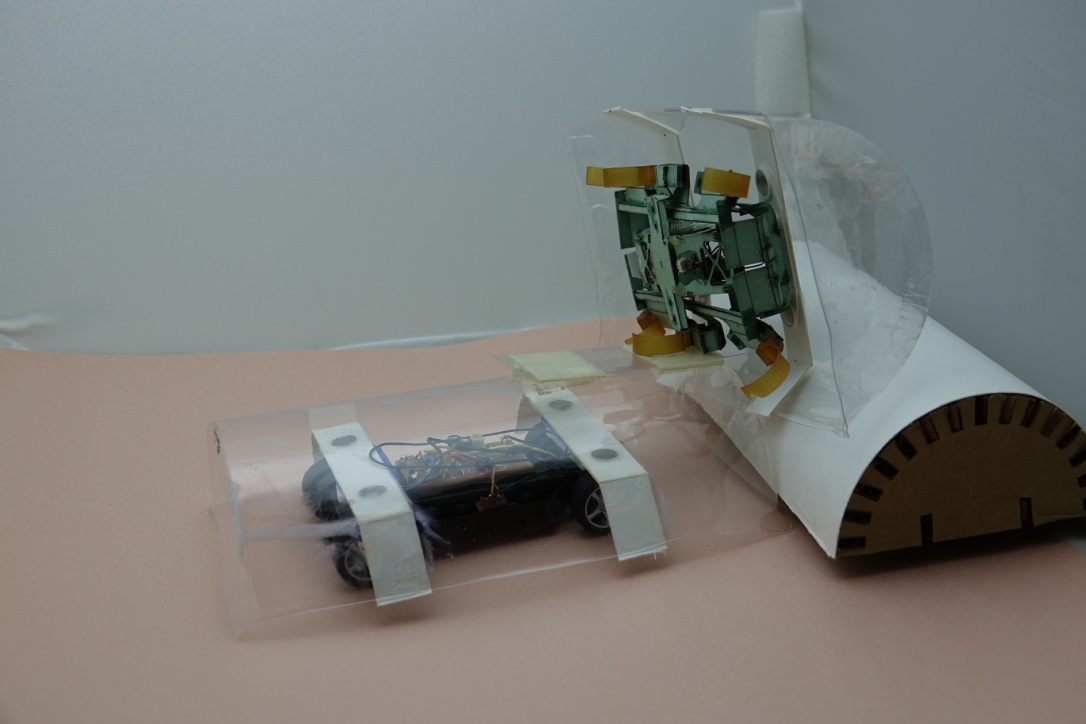
\includegraphics[width=0.16\textwidth]{KinPanel5.jpg}
  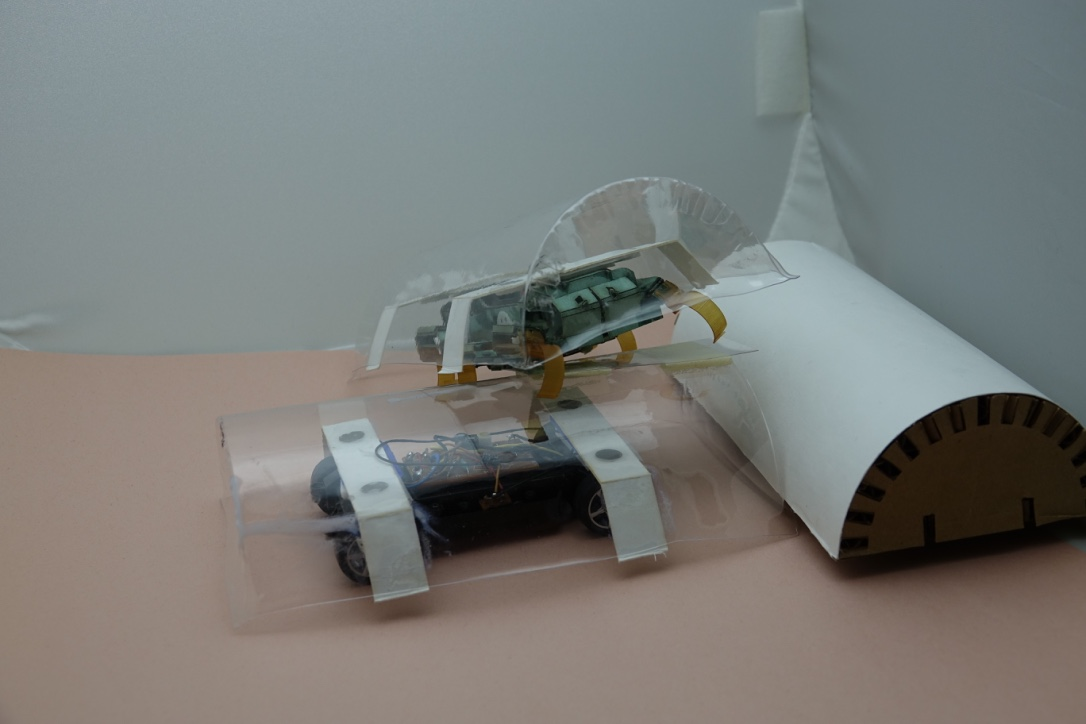
\includegraphics[width=0.16\textwidth]{KinPanel6.jpg}
  \caption{\label{fig:KinematicFlipRealLife}Kinematic Progression of Cooperative Righting}
\end{figure}

Each configuration of the two compatriot robots exerts force closure on the pronated robot, and the sequence of configurations moves the pronated robot from prone to upright.
Unfortunately, when these kinematic frames are chained over time, unmodeled dynamics come into play.
When \textit{push comes to shove} the pushing robot cannot exert sufficient force to progress through the kinematic frames.

\begin{figure}[ht]
  \centering
  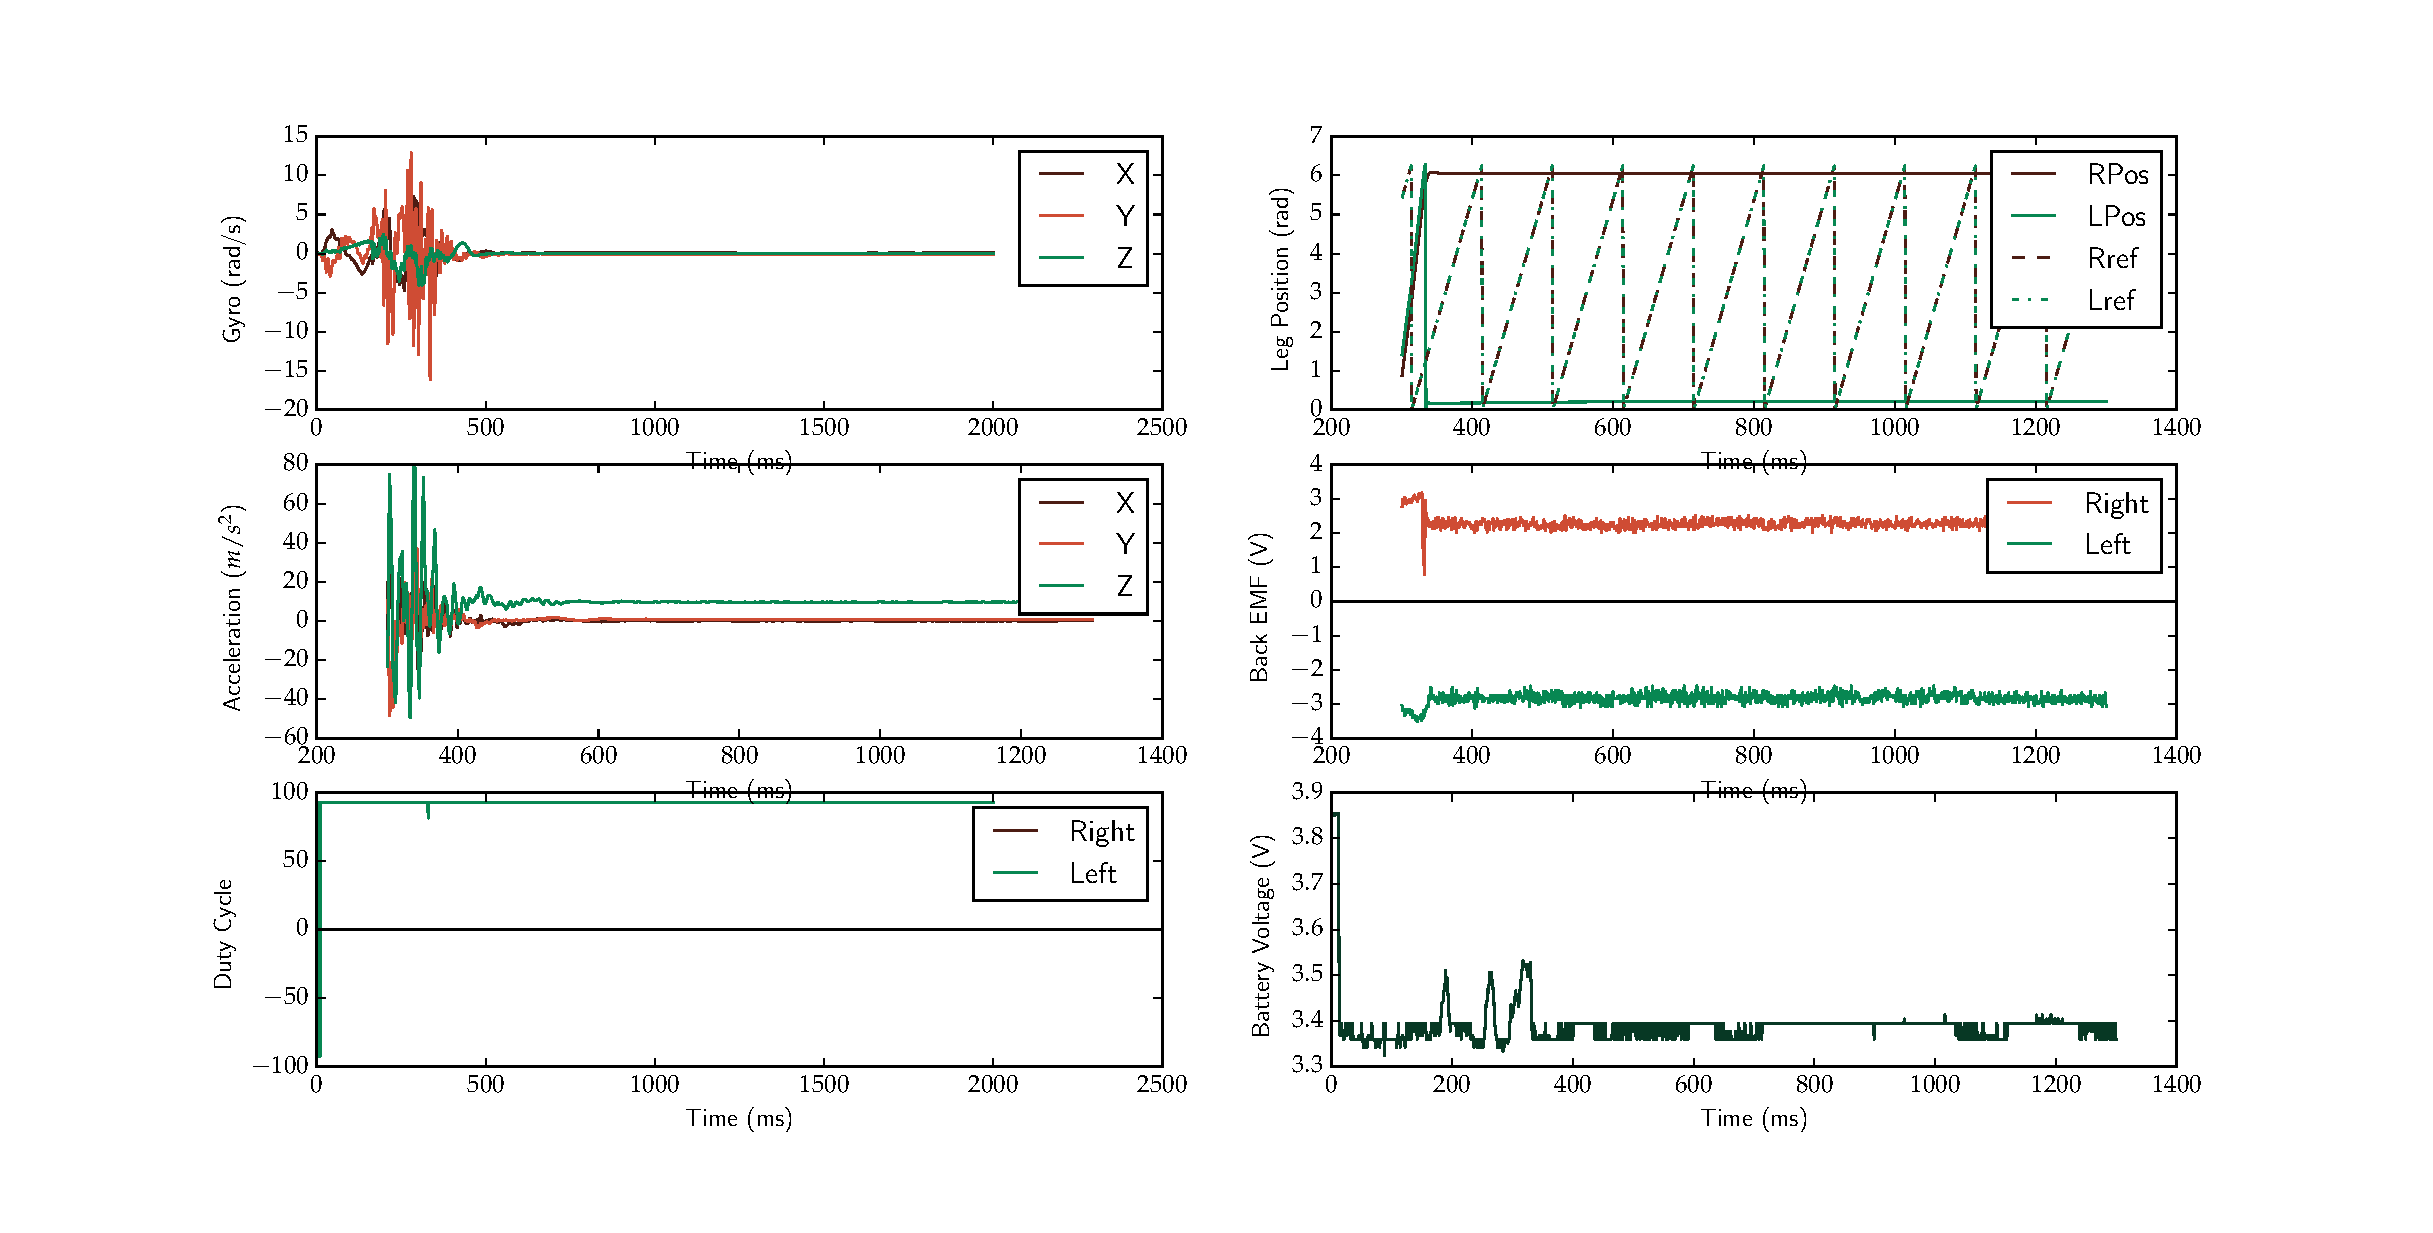
\includegraphics[width=\textwidth]{JammedTelemetry.eps}
  \caption{\label{fig:JammedKinFlipTelemetry}Telemetry of Jammed Pushing Compatriot Robot}
\end{figure}

We will analyze this failure using quasi-static analysis in the next section.

\section{Force Analysis \label{sec:KinForces}}
From the free-body diagram in Fig. \ref{fig:KinFreebody} quasi-static force equilibrium equations are:

\begin{align}
  P + F \sin(\alpha + \phi) - N \cos(\alpha + \phi) = 0
  \label{eq:KinQSX}
\end{align}

\begin{align}
  L + F \cos(\alpha + \phi) + N \sin(\alpha + \phi) = mg
  \label{eq:KinQSY}
\end{align}

\begin{align}
  F r \sin(\theta + \phi + \alpha) - N r \cos(\theta + \phi + \alpha) = mg r \cos(\theta)
  \label{eq:KinTorque}
\end{align}

We also assume that the two shells are sliding:

\begin{align}
  F = \mu N
  \label{eq:KinFriction}
\end{align}

where $\mu$ denotes here the coefficient of friction between the two shells.

\begin{comment}
For the sake of notational brevity, we compact the trigonometric expressions to the following:

\begin{align}
  a &= \cos(\theta + \phi) \\
  b &= \sin(\theta + \phi) \\
  c &= \cos(\alpha) \\
  d &= \sin(\alpha) \\
  e &= \cos(\phi) \\
  f &= \sin(\phi)
\end{align}

Substituting Eq. \ref{eq:KinFriction} into Eq. \ref{eq:KinTorque} and solving for the normal force along the shell contact yields:

\begin{align}
N = \frac{c m g}{\mu (1+ac-bd) + (bc+ad)}
\end{align}

Further substituting this expression into Eqs. \ref{eq:KinQSX} and \ref{eq:KinQSY} results in expressions for the push forces needed from the perpendicular hinge compatriot:

\begin{align}
P = ( (ce-df) - (cf+de)\mu ) \frac{c m g}{\mu (1+ac-bd) + (bc+ad)}
\end{align}
and
\begin{align}
L = ( (cf+de) - (ce-df)\mu )\frac{c m g}{\mu (1+ac-bd) + (bc+ad)}
\end{align}
\end{comment}

Substituting Eq. \ref{eq:KinFriction} into Eq. \ref{eq:KinTorque} and solving for the normal force along the shell contact yields:

\begin{align}
N = \frac{\cos(\theta) m g}{\mu (1+\cos(\theta + \phi + \alpha)) + \sin(\theta + \phi + \alpha)}
\end{align}

Further substituting this expression into Eqs. \ref{eq:KinQSX} and \ref{eq:KinQSY} results in expressions for the push forces needed from the perpendicular hinge compatriot:

\begin{align}
P = ( \cos(\alpha+\phi) + \mu \sin(\alpha+\phi) ) \frac{\cos(\theta) m g}{-\mu (1+\cos(\theta + \phi + \alpha)) + \sin(\theta + \phi + \alpha)}
\end{align}
and
\begin{align}
L = ( -\sin(\alpha+\phi) + \mu \cos(\alpha+\phi) ) \frac{\cos(\theta) m g}{-\mu (1+\cos(\theta + \phi + \alpha)) + \sin(\theta + \phi + \alpha)} + mg
\end{align}

\begin{comment}
These forces are plotted as a function of distance in Fig. \ref{fig:KinForces}

\begin{figure}[ht]
\centering
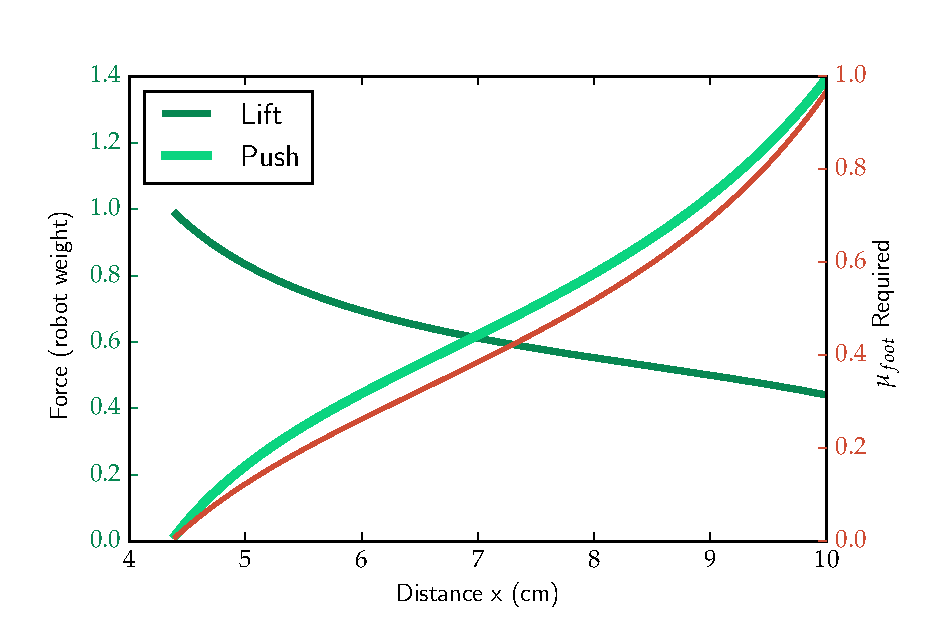
\includegraphics[width=0.5\textwidth]{KinPushForces2.eps}
\caption{\label{fig:KinForces}Push Forces for Kinematic Flip (measured as multiples of robot weight)}
\end{figure}

Note that when the push begins at $x=10 cm$, the required coefficient of friction between ground and robot is higher than the actual foot-ground coefficient range of $0.5$ to $0.7$.
%TO DO: The push doesn't begin at 10 cm. It begins at 14.9 cm as dictated by w=r+sqrt(4r^2 - h) where h = 3cm (measured).
\end{comment}

Note that the expressions for $P$ and $L$ both have a dividing term

$$-\mu (1+\cos(\theta + \phi + \alpha)) + \sin(\theta + \phi + \alpha)$$

which arises from their dependence on $N$ with the term being proportional to the moment arm of $N+F$ around the hinge.
For every righting procedure between two circles, there will always be a point where the line of action of $N+F$ (which forms an angle $\psi = \tan^-1(1/\mu)$ to the line connecting the two circles' centers) will intersect the hinge, resulting in a zero moment arm and:

$$-\mu (1+\cos(\theta + \phi + \alpha)) + \sin(\theta + \phi + \alpha) = 0$$

This arithmetical breakdown from dividing by zero arises from our a breakdown in our assumptions; namely, that the shells are always sliding against each other.
Instead, we find the shells \textbf{must be} sticking.
This was the observed problem in the robotic experiments that caused the jamming seen in Fig. \ref{fig:JammedKinFlipTelemetry}.
%TODO: Why doesn't this jam when I use the infinitely-powerful actuator (my arm) to move the robots together?

\chapter{Quasi-static Flip Method}
\begin{figure}[ht]
\centering
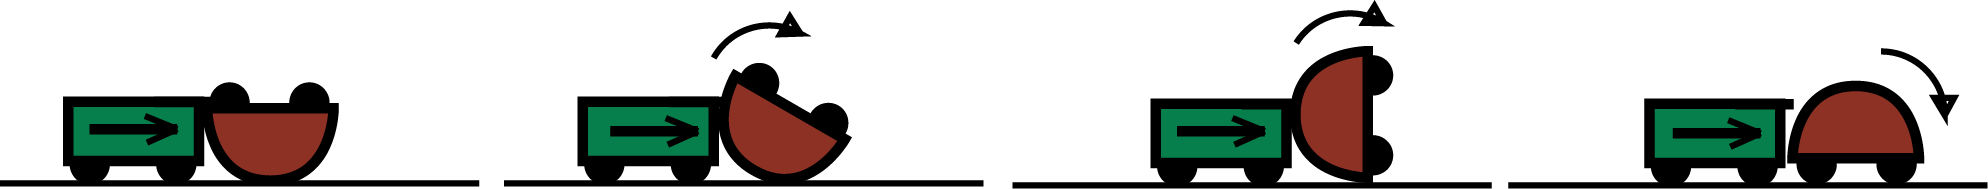
\includegraphics[width=1.0\textwidth]{QuasiStatic_CoopCartoon.png}
\end{figure}

Kinematic manipulation design focuses on the pure geometry of the problem.
As we witnessed, this myopic physics treatment neglects important possible confounds like friction.
In Section \ref{sec:KinForces} we saw that despite working kinematically, it does not work quasi-statically as the friction force causes the push to jam.

The beauty of engineering is that we can convert this confounding force into a useful force.
By accounting for quasi-static forces like friction in our design we can create a more versatile cooperative locomotive maneuver.
The friction force can replace the second finger in creating the moment couple, thereby only requiring one compatriot robot.

Our shell design for the quasi-static flip is inspired by that most classic of inventions: the wheel.
We will use a semi-circular prism with a high friction tire attached.
The maneuver only requires the compatriot robot to run into the prone robot; the auto-alignment (from Sec. \ref{sec:Reuleaux}) will take care of the rest.

This design is also inspired by domed turtle shells. Domokos et. al \cite{domokos2008geometry} studied how turtles' shell shapes allow them to right themselves when tipped over.

\section{Newtonian Analysis}
The main breaking points for successful quasi-static flipping maneuvers are having the requisite pushing force capacity and sufficient traction between the prone robot's shell and the ground.
To analyze these two variables a simple quasi-static force analysis is sufficient.

For this pushing maneuver to succeed, both ``fingers'' must have sufficient force capacity: both the compatriot robot's push and the ground's friction force.
These can be readily obtained by an quasi-static Newtonian analysis.

\begin{figure}[ht]
\centering
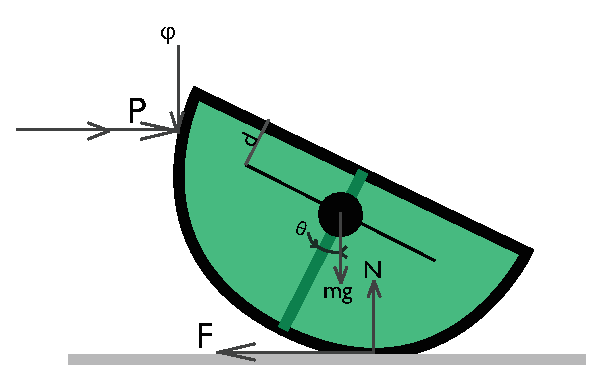
\includegraphics[width=0.5\textwidth]{QS_FreeBodyDiagram2.eps}
\caption{\label{f:QS_FBD}Freebody Diagram for Quasi-static Newtonian Analysis}
\end{figure}

We extract the equilibrium equations from the free-body diagram in Fig. \ref{f:QS_FBD} as:

\begin{align}
  F = P \label{e:QSF_x} \\
  N = mg + B \label{e:QSF_y} \\
  P d \cos(\theta) + F(r - d \cos(\theta)) - N d \sin(\theta) - B (r - d \sin(\theta)) = 0 \label{e:QSF_o}
\end{align}

We also assume the prone robot's shell is sliding along the compatriot robot's front at all times (no lip for catching and hinging, unlike the Kinematic Flip's design):

\begin{align}
  B = \mu P \label{e:QSF_plowFriction}
\end{align}

\subsection{Push Force Requisite}
Manipulating Eq. \ref{e:QSF_o} and substituting (in order) Eqs. \ref{e:QSF_x}, \ref{e:QSF_y}, \ref{e:QSF_plowFriction}

\begin{align}
  0 &= P d \cos(\theta) + P(r - d \cos(\theta)) - N d \sin(\theta) - B (r - d \sin(\theta))
  \\&= Pr - N d \sin(\theta) - B (r - d \sin(\theta))
  \\&= Pr - (mg + B) d \sin(\theta) - B (r - d \sin(\theta))
  \\&= Pr - mg d \sin(\theta) - B r
  \\&= (P - B)r - mg d \sin(\theta)
  \\&= (1-\mu) P r - mg d \sin(\theta)
\end{align}

Solving for $P$ yields:

\begin{align}
  P = \frac{mg}{1-\mu} \frac{d}{r} \sin(\theta)
\end{align}

Which means that the pushing robot needs to be able to apply at least the maximum push force required throughout the manipulation:

\begin{align}
  \text{push capacity} \geq P_{max} = \max_\theta \frac{mg}{1-\mu} \frac{d}{r} \sin(\theta) = \frac{mg}{1-\mu} \frac{d}{r}
\end{align}

Note that any friction between the pusher's front surface and the pronated robot's shell increases the required push force.
The requisite push force goes to infinity as $\mu$ approaches unity.
Therefore, we seek to make the friction between the two shells as low as possible.
We will also need a fairly strong pushing robot.

\subsection{Friction Requisite}
For this analysis we desire (and assume) that the prone robot is rolling without slip along the ground, thereby constraining the friction force inside the cone described by:

\begin{align}
  F \leq h N \label{e:QSF_groundFriction}
\end{align}

where $h$ is the friction coefficient between the pronated shell and the ground.
Plugging Eq. \ref{e:QSF_x} into the left-hand side of Eq. \ref{e:QSF_groundFriction} and Eq. \ref{e:QSF_y} into the right-hand side (along with Eq. \ref{e:QSF_plowFriction}) yields:

\begin{align}
  P \leq \frac{hmg}{1-h\mu} \label{e:QSF_pushConstraint1} \hspace{5mm} \forall \theta
\end{align}

The tightest bound will be at the $\theta$ when push force is maximized $P_{max}$:

\begin{align}
  P_{max} = \frac{mg}{1-\mu} \frac{d}{r} &\leq \frac{hmg}{1-h\mu} \\
  \frac{1}{1-\mu} \frac{d}{r} &\leq \frac{h}{1-h\mu}
  \label{e:gndFrictionReq}
\end{align}

when we assume the shell-shell contact is frictionless the requirement on the shell-ground contact reduces to:

\begin{align}
  \frac{d}{r} &\leq h
\end{align}

If the ground friction is insufficient the prone robot will only roll up to a critical angle $\theta_{break}$.
At that point the friction constraint is exactly met, the prone robot will begin to slide, and any further pushing will only result in sliding instead of rolling.
To avoid this failure mode, we add a Santoprene tire at both ends of the robot shell, thereby boosting shell-ground contact $h$ while leaving a section of the shell smooth for low friction shell-shell contacts $\mu$.

\section{Hamiltonian Analysis \label{sec:QS_HamAnalysis}}
We have now proposed a new flipping strategy predicated on quasi-static forces; filling the quasi-static niche in Mason's taxonomy of manipulation \cite{MasonMORMBook}.
With a Newtonian (or, as Mason would call quasi-static analysis, Aristotelian) analysis we have prescribed the conditions for a successful cooperative righting maneuver.
In this section we analyze the performance of the flip in time, extending to a dynamic investigation.
We will use a Hamiltonian formulation to model this constrained dynamic system (rolling without slip reduces the problem from three states to one state).
Furthermore, we will use this energetic analysis to argue that the semi-circle is optimal for our problem.

The VelociRoACH platform is optimized for speed and robustness, not torque and stability (which would be what we need for stable pushing).
Accordingly our shell design for this platform must aim to minimize the requisite maximum power transfer necessary (throughout the maneuver).
This can be analyzed by the change in potential energy as the prone robot undergoes rotation.
To this end, let us find the gravitational potential energy of a tilted robot at each angular configuration.
We narrow our focus of shell shape design to the class of 3D shapes with elliptical cross sections in the plane of rotation.
This focusing is motivated by analogy to the wheel and the intuition of avoiding corners.

\begin{figure}[ht]
\centering
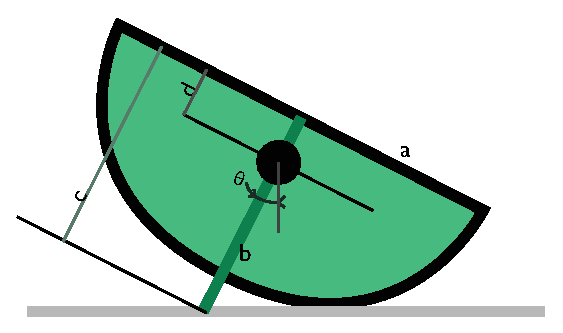
\includegraphics[width=0.5\textwidth]{QS_EnergyAnalysis.eps}
\caption{\label{f:QS_energyGeometry}Geometric Diagram for Tilted Ellipse Energy Analysis}
\end{figure}

Consider Fig. \ref{f:QS_energyGeometry} where $a,b$ are the ellipse's major and minor axes' lengths.
The energy at a given tilt angle $\theta$ will be:

\begin{align}
  E(\theta) =
    \begin{cases}
      mg (c(\theta)-d) \cos(\theta), & \text{if}\ \theta < \frac{\pi}{2} \\
      mg (a \sin(\theta) - d \cos(\theta) ), & \text{if}\ \frac{\pi}{2} \leq \theta < \frac{\pi}{2} + \tan^{-1}(d/a)
    \end{cases}
  \label{eq:QSEnergy}
\end{align}

where $c$ is the minor-axis intercept of the unique tangent line to the semi-ellipse with angle $\theta$ (this tangent defines the ground contact point):

\begin{align}
  c(\theta) \doteq \sqrt{a^2 \tan^2(\theta) + b^2}
\end{align}

\begin{figure}[ht]
  \centering
  \begin{subfigure}[t]{0.45\textwidth}
    \centering
    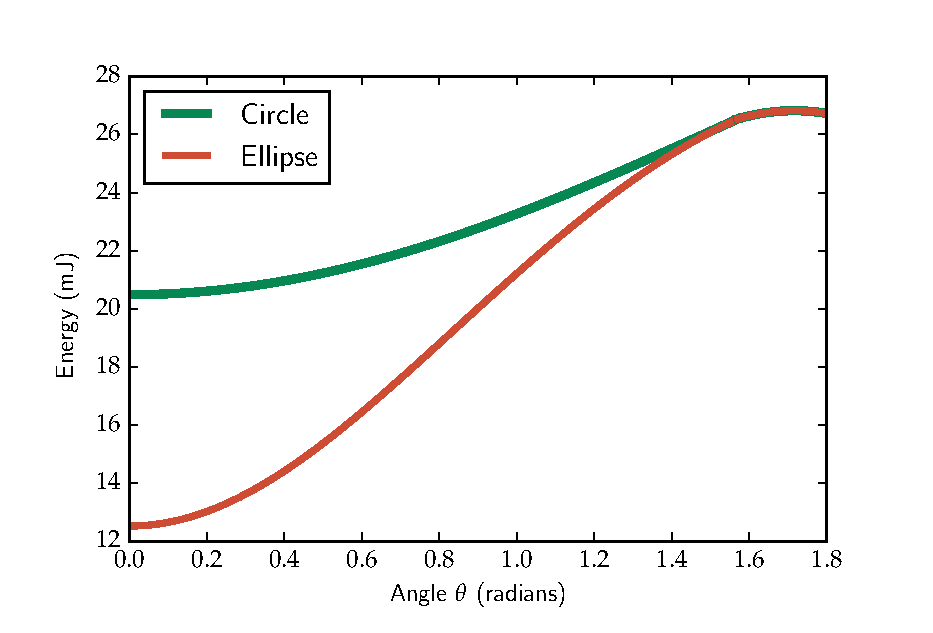
\includegraphics[width=1.0\textwidth]{EnergyLandscape.eps}
    \caption{\label{fig:QSEnergy}Energy Landscape over Prone Robot's Angle as described in Eq. \ref{eq:QSEnergy}}
  \end{subfigure}
  \hfill
  \begin{subfigure}[t]{0.45\textwidth}
    \centering
    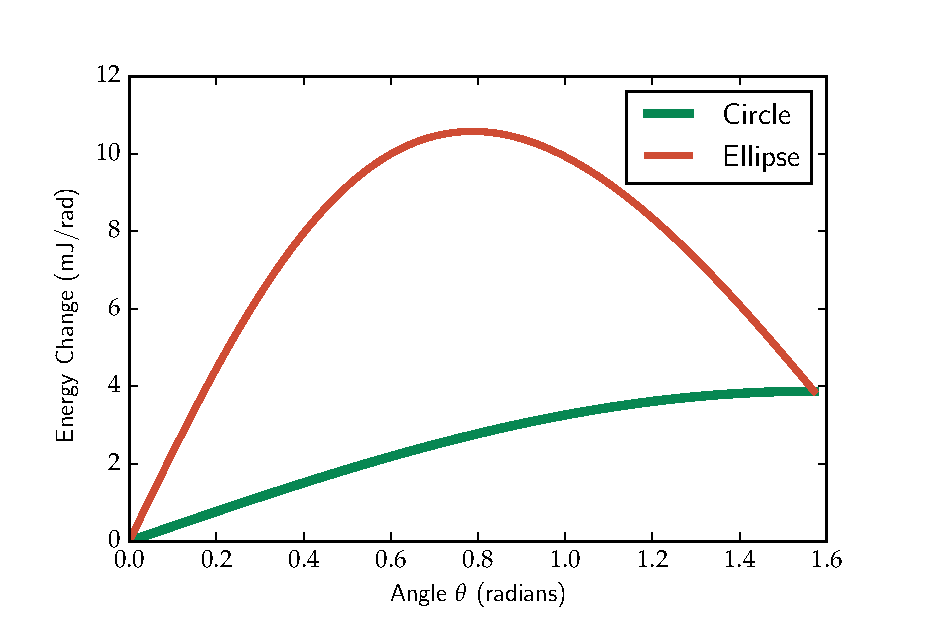
\includegraphics[width=1.0\textwidth]{dEnergyLandscape.eps}
    \caption{\label{fig:QSdEnergy}Energy Differential plotted against Angle as described in Eq. \ref{eq:QSdEnergy}}
  \end{subfigure}
\end{figure}

So that the change in energy required for progression along rotation $\theta$ is:

\begin{align}
  \frac{dE}{d\theta} =
  \begin{cases}
    mg ( (a^2 - b^2) \frac{\sin(\theta)}{\sqrt{a^2 \tan^2(\theta) + b^2}} + d \sin(\theta) ), & \text{if}\ \theta < \frac{\pi}{2} \\
    mg (a \cos(\theta) + d \sin(\theta) ), & \text{if}\ \frac{\pi}{2} \leq \theta < \frac{\pi}{2} + \tan^{-1}(d/a)
  \end{cases}
  \label{eq:QSdEnergy}
\end{align}

This energy differential over position describes how much work must be performed, or how much force is required.
It is plotted in Fig. \ref{fig:QSdEnergy}

Note that the maximum force for pushing a circle is non-decreasing and is maximum at $\theta = \pi/2$ (this will be confirmed again in the below force analysis).
In contrast, the maximum force for pushing an ellipse is much larger and occurs in the middle of the pushing maneuver.
We will see this larger energy requisite manifest as significantly slower pushing maneuvers when operating on ellipses.

\section{Experimental Results}
\begin{figure}[ht]
\centering
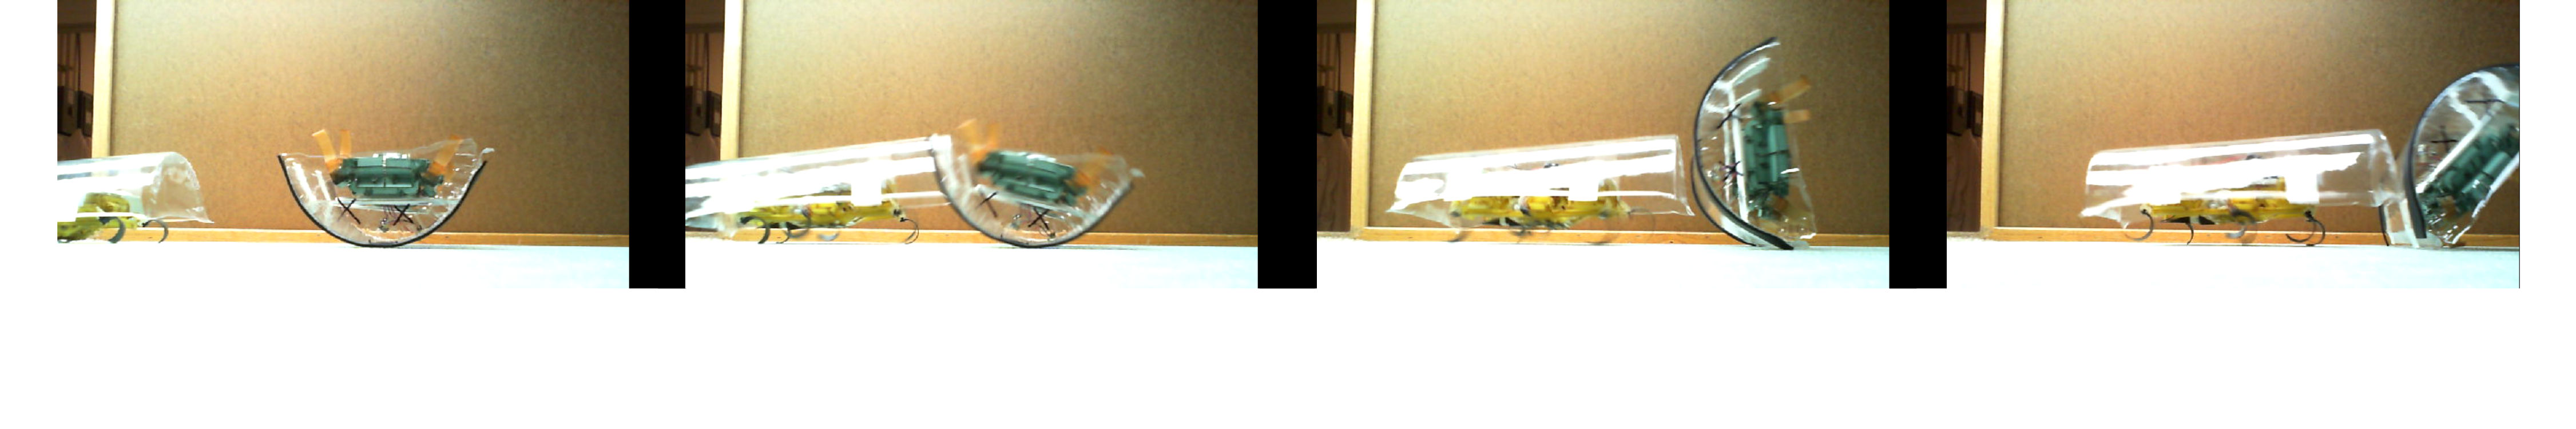
\includegraphics[width=1.0\textwidth]{QSFlipStrip3.png}
\caption{Frame sequence of RoACH team performing quasi-static cooperative righting maneuver on styrofoam}
\end{figure}

The VelociRoACH robot was equipped with a cylindrical shell and set to walk forwards for 2 seconds after being setup and aimed at another pronated VelociRoACH robot.
The experimental results are summarized in Tbl. \ref{tbl:results}
The flipping maneuver successfully 26 times out of 30 trials. Two of the failures were due to the pushing robot deflecting away from the prone target upon impact.
The other two failures were only due to not running the robot long enough (only 2 seconds).
Both failures will be easily fixed with the addition of a heading controller and flip end-condition check, respectively.
These features were not implemented in this base test for sake of repeatability and to avoid a changing control signal that would confound power estimates.

\begin{table*}[tb]
% increase table row spacing, adjust to taste
\renewcommand{\arraystretch}{1.1}
\caption{Results Table}
\label{tab:Results}
\centering
\begin{tabular}{l l c c}
\hline
Condition Icon\label{tbl:results} & Condition Description & Successes & Avg. Righting Time (ms) \\
\hline
\raisebox{-\totalheight/2}{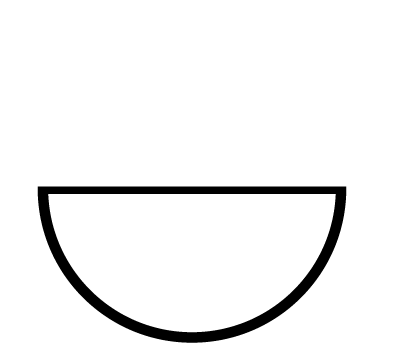
\includegraphics[width=0.05\textwidth]{CircleIcon.png}} & Semi-circular Prism & 26/30 (87\%) & 405.2 ms \\
\raisebox{-\totalheight/2}{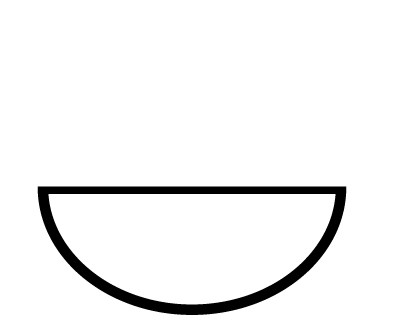
\includegraphics[width=0.05\textwidth]{EllipseIcon.png}} & Semi-elliptical Prism & 15/20 (75\%) & 512.6 ms \\
\hline
\raisebox{-\totalheight/2}{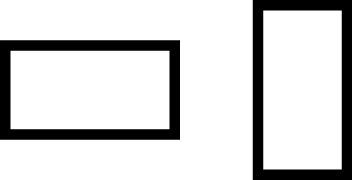
\includegraphics[width=0.05\textwidth]{0Align.png}} & Prism, Straight (0 degree) Alignment & 26/30 (87\%) &  \\
\raisebox{-\totalheight/2}{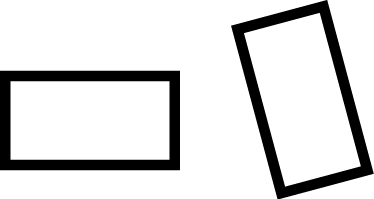
\includegraphics[width=0.05\textwidth]{30Align.png}} & Prism, Scant (30 degree) Alignment & 5/5 (100\%) &  \\
\raisebox{-\totalheight/2}{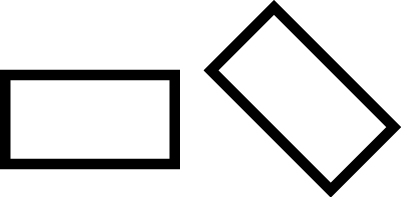
\includegraphics[width=0.05\textwidth]{45Align.png}} & Prism, Scant (45 degree) Alignment & 5/5 (100\%) &  \\
\raisebox{-\totalheight/2}{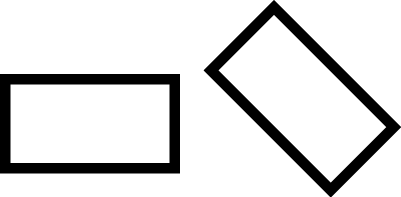
\includegraphics[width=0.05\textwidth]{60Align.png}} & Prism, Scant (60 degree) Alignment & 2/5 (40\%) &  \\
\raisebox{-\totalheight/2}{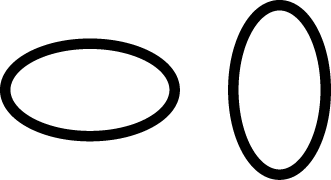
\includegraphics[width=0.05\textwidth]{EllipEllipAlign.png}} & Ellpisoidal, Straight (0 degree) & 0/5 (0\%) & \\
\hline
\raisebox{-\totalheight/2}{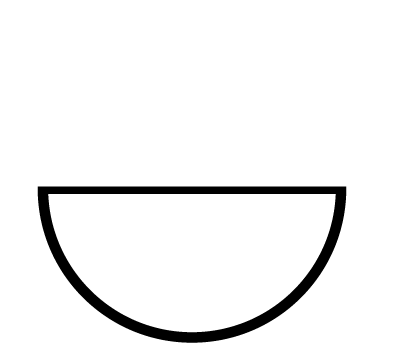
\includegraphics[width=0.05\textwidth]{CircleIcon.png}} & Rubberized Prism & 26/30 (87\%) & 405.2 ms \\
\raisebox{-\totalheight/2}{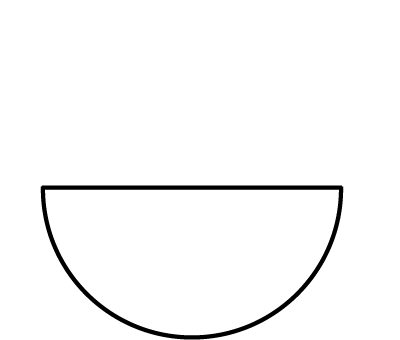
\includegraphics[width=0.05\textwidth]{BareCircleIcon.png}} & Bare Prism & 0/5 (0\%) &  \\
\hline
\end{tabular}
\end{table*}

\subsection{Ground Friction Requisite}
As shown in Eq. \ref{e:gndFrictionReq} a minimum shell-ground friction coefficient is necessary to successfully perform a quasi-static flip.
This was tested experimentally by varying the friction coefficient using the added tractive strips made of Santoprene rubber.
The successful design condition discussed above (with the 26/30 success rate) used Santoprene strips.
When these strips were removed the bare plastic failed to grip the ground and 5/5 flip attempts failed.
This manifested as 3/5 pushes failing due to the prone robot simply skittering away from the pusher, and 2/5 pushes failing after the prone robot twisted (in yaw) away from the push thereby deflecting the pusher off to the side.

\subsection{Footprint Alignment}
In Section \ref{sec:Molds} we chose to narrow designs to prismatic extrusions of 2D shapes, asserting that secondary curvature was actually undesirable.
That assertion was tested experimentally by varying the entry angle of the prismatic robots to assess alignability and was contrasted with the poor experimental alignment performance of ellipsoidal shells.

As demonstrated in subsection \ref{sec:Reuleaux} via Reuleaux's method, robots with the prismatic design (rectangular footprint) will self-align when pressed together.
When initialized with alignment (=zero degree offset) the robots stayed align in 28/30 trials.
When initialized with 30 degree, 45 degree, or 60 degree offsets the alignment succeeded in 5/5, 5/5 and 2/5 trials respectively.
Therefore, past a 45 degree offset the self-alignability of the shells drops off, instead yawing the robots into the parallel (non-engaged) configuration.

We then tested pushing with ellipsoidal designs (elliptical footprint).
Even when initialized already aligned the pusher deflected away from the target robot immediately upon contact (successful alignment in 0/10 trials).
This is easily understood from a classical grasping standpoint; the elliptical footprint of the pushing robot contacts the target along its unstable major axis.
This observation also aligns with the design reasoning for why previous shell iterations for the VelociRoACH used ellipsoids: terradynamic streaming.
The goal of ``terradynamic streaming'' is to create exterior hulls for the robot that will slip past obstacles upon collision.
As attested to in this experiment, the ellipsoidal hull is excellent at deflecting away from obstacles.
This selfsame characteristic becomes undesirable when we instead need the robot to transfer force to obstacles it engages.




\chapter{Dynamic Flip Method}
\begin{figure}[ht]
\centering
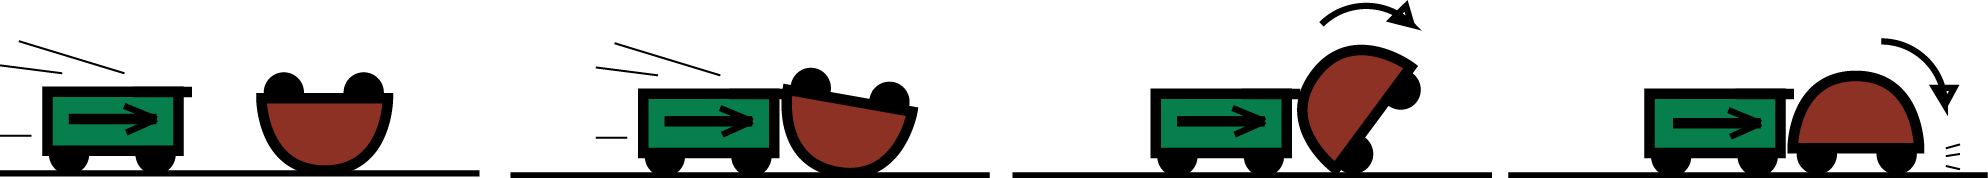
\includegraphics[width=1.0\textwidth]{Dynamic_CoopCartoon.png}
\caption{Cartoon of ``Dynamic'' Cooperative Flip Technique \label{fig:DynCartoon}}
\end{figure}
The final flipping method eschews reliance upon friction by replacing it (in its role of invisible second finger) with the more ubiquitous inertial pseudo-force.
This flipping method is purely ballistic, and by relying on dynamic effects fills the last niche in Mason's taxonomy of manipulation \cite{MasonMORMBook}.
Indeed, the VelociRoACH platform is optimized for speed over pushing strength (as was required for the quasi-static flipping method), so this dynamic flipping method plays to its strengths.
The design challenge will be in ensuring that the transferred kinetic energy from compatriot to pronate is stored as rotational kinetic energy instead of translational kinetic energy.

\section{Hamiltonian Analysis}
If friction can be relied upon, then the system collapses from three states to one thanks to the rolling constraint.
The Hamiltonian for this dynamic system will be the same as that explored in Sec. \ref{sec:QS_HamAnalysis}:

\begin{align}
  H(p,\theta) = U(\theta) + T(p,\theta) =
\end{align}

However, the strength of this more dynamic flipping scheme (purely ballistic) is that it works even in absence of friction.
Without the rolling constraint, our system maintains all three degrees of freedom.
The Hamiltonian problem becomes fairly simple:

\begin{align}
  H(p,z) = U(z) + T(p) = m g h + \frac{1}{2 m} p^2
\end{align}

Indeed, we get discover a basic success condition by evaluating the Hamiltonian at the first three snapshots shown in Fig. \ref{fig:DynCartoon} (and assuming energy transfer is purely elastic and optimally transferred to rotational kinetic energy):

\begin{align}
H_0 = \frac{1}{2} m_1 v_1^2  \\
H_1 = \frac{1}{2} I_2 \omega_2^2  \\
H_2 = m_2 g \sqrt{d^2+r^2} \\
\rightarrow v_1 &= \sqrt{\frac{m_2}{m_1}g \sqrt{d^2+r^2}} \\
 v_1 &= \sqrt{g \sqrt{d^2+r^2}}
\end{align}

We need the initial velocity of the ballistic compatriot to be at least $\sqrt{g \sqrt{d^2+r^2}}$ to hope to crest the potential barrier.
In reality we'll need the initial velocity to be greater than that to deal with leakages to translational kinetic energy (slippage) and inelastic loss of impact.

\section{Experimental Results}
No results

\chapter{Conclusion: Discussion and Future Work}
To be written second to last.

\section{Acknowledgements}
Many thanks to Carlos Casarez for his indispensable advice on experimental design and analyses as well as general direction on where to take this project.

\bibliographystyle{plain}
\bibliography{manipulation}

\end{document}
